%WTW124.tex
% This file is part of the WTW124 course material.
\documentclass[11pt]{article}
\usepackage{amsmath, amssymb, amsthm}
\usepackage{xcolor}
\usepackage[most]{tcolorbox}
\usepackage{geometry}
\geometry{margin=1in}
\usepackage{graphicx}
\usepackage{enumitem}
\usepackage{tikz}
\usepackage{tikz-3dplot}
\usepackage{multicol}
\usepackage{lmodern}
\usepackage{setspace}
\usepackage{titlesec}
\usepackage{fancyhdr}
\usetikzlibrary{arrows.meta}
\usepackage{array}
\usepackage{booktabs}
\usepackage{hyperref}



\setlength{\parindent}{0pt}



% Custom environments
\newtcolorbox{definitionbox}{colback=green!10!white,colframe=green!50!black,title=Definition}
\newtcolorbox{remarkbox}{colback=red!5!white,colframe=red!75!black,title=Remark}
\newtcolorbox{examplebox}{colback=blue!5!white,colframe=blue!75!black,title=Example}
\newtcolorbox{theorembox}{colback=orange!10!white,colframe=orange!80!black,title=Theorem}
\newtcolorbox{proofbox}{colback=yellow!10!white,colframe=yellow!80!black,title=Proof}
\newtcolorbox{notebox}{colback=gray!10!white,colframe=black,title=Take Note!}
\newtcolorbox{exercisebox}{colback=purple!10!white,colframe=purple!80!black,title=Exercises}
\newtcolorbox{propositionbox}{colback=cyan!10!white,colframe=cyan!80!black,title=Proposition}


\begin{document}

\begin{titlepage}
    
\begin{tikzpicture}[remember picture,overlay]
        \draw[line width=1pt]
            ([xshift=1in,yshift=-1in]current page.north west) rectangle
            ([xshift=-1in,yshift=1in]current page.south east);
    \end{tikzpicture}

    \vspace*{4cm}

    \begin{center}
        {\Huge \bfseries WTW 124}\\[0.5cm]
        {\Huge \bfseries Mathematics}\\[1.5cm]
        
        \rule{\textwidth}{0.4pt}\\[1.5cm]

    
        {\normalsize \textit{Open Course Notes}}\\[1.5cm]
        {\normalsize Based on \textit{\textbf{Mathematics 124 Course Notes}}}\\[3cm]

        % Add the link here
        {\footnotesize Available at \url{https://tinyurl.com/wtw124-git}}
    \end{center}
\end{titlepage}

\tableofcontents
\newpage


\section{Vectors and a Model for Space}


\textbf{Introduction}
\\
Imagine you're standing in a rectangular room. To describe the exact position of any point in the room, say, 
where a fly is hovering, we can use three numbers. These numbers form an ordered triple:

\[
\langle x_1, x_2, x_3 \rangle
\]
\begin{itemize}
\item $x_1$ is the distance from one wall,
\item $x_2$ is the distance from the opposite wall (not the same one as $x_1$),
\item $x_3$ is how high the point is from the floor.
\end{itemize}


These values give us a simple way to describe positions in 3D space using real numbers. 
This forms the basis of vectors in $\mathbb{R}^3$.
\begin{center}
  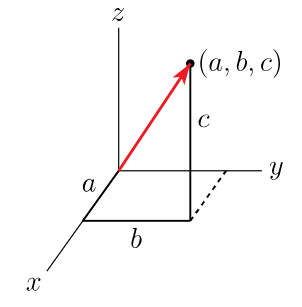
\includegraphics[width=0.7\textwidth]{figures/Vector.png}
\end{center}



\newpage

\subsection{Algebraic Vectors and Vector Algebra}

\subsubsection{Algebraic Vectors}


In this section, we formalise the ideas presented in the introduction.
At this point our definitions and theorems are purely mathematical, and have no connection
with the physical world.

\begin{definitionbox}
\textbf{Algebraic Vectors}

Let $n$ be any number in $\mathbb{N}$. An algebraic vector with $n$ components is an ordered set:
\[
\bar{x} = \langle x_1, x_2, ..., x_n \rangle, \quad \text{where } x_i \in \mathbb{R}
\]
These numbers are called the \textit{components} of $\bar{x}$.
\end{definitionbox}

\begin{definitionbox}
\textbf{Notation}

The set of all vectors with $n$ real-number components is denoted by $\mathbb{R}^n$.
\end{definitionbox}

\begin{examplebox}
\begin{itemize}
\item $\bar{x} = \langle 1, 2, -3 \rangle \in \mathbb{R}^3$
\item $\bar{y} = \langle -2, 0.7, 1.1, 0.2 \rangle \in \mathbb{R}^4$
\item $\bar{z} = \langle -1, 2, 3, -3 \rangle \in \mathbb{R}^4$
\end{itemize}
\end{examplebox}

\begin{definitionbox}
\textbf{Vector Equality}

Two vectors $\bar{x} = \langle x_1, x_2, ..., x_n \rangle$ and $\bar{y} = \langle y_1, y_2, ..., y_n \rangle$ are equal if and only if:
\[
x_1 = y_1, \quad x_2 = y_2, \quad ..., \quad x_n = y_n
\]
\end{definitionbox}

\begin{remarkbox}
Vectors are \textbf{ordered sets}. They are only equal if they have the same number of components and each corresponding component is equal.
\end{remarkbox}

\begin{examplebox}
The vectors $\bar{x} = \langle 1, 2, -3 \rangle$ and $\bar{y} = \langle 1, -3, 2 \rangle$ in $\mathbb{R}^3$ are not equal, since $x_3 = -3 \neq 2 = y_3$.

Also, let $\bar{w} \in \mathbb{R}^4$. Then the algebraic vectors $\bar{z} = \langle 1, 1, 1 \rangle$ and $\bar{w} = \langle 1, 1, 1, 1 \rangle$ are not equal, since $\bar{z} \in \mathbb{R}^3$ and $\bar{w} \in \mathbb{R}^4$.

\end{examplebox}

\newpage

% Section 2
\subsubsection{Algebraic Vector Operations}


The set $\mathbb{R}^n$ is equipped with algebraic operations in a natural way.
We can add vectors, multiply them by scalars, and subtract them.
These operations are defined as follows:
\begin{definitionbox}
\textbf{Vector Addition}

If $\bar{x}, \bar{y} \in \mathbb{R}^n$, then:
\[
\bar{x} + \bar{y} = \langle x_1 + y_1, x_2 + y_2, ..., x_n + y_n \rangle
\]
\end{definitionbox}

\begin{definitionbox}
\textbf{Scalar Vector Multiplication}

If $c \in \mathbb{R}$ and $\bar{x} \in \mathbb{R}^n$, then:
\[
c\bar{x} = \langle cx_1, cx_2, ..., cx_n \rangle
\]
\end{definitionbox}

\begin{notebox}
\textbf{Terminology...}

Some textbooks say that this is not the same as scalar \textit{product}, which refers 
to the dot product of two vectors. 
For our purposes we shall refer to the above definition as scalar vector \textit{multiplication}.
\end{notebox}

\begin{definitionbox}
\textbf{Zero Vector}

The \textit{zero vector} in $\mathbb{R}^n$ is:
\[
\bar{0} = \langle 0, 0, ..., 0 \rangle
\]
\end{definitionbox}

\begin{definitionbox}
\textbf{Additive Inverse of a Vector}

For $\bar{x} \in \mathbb{R}^n$, the additive inverse is:
\[
-\bar{x} = \langle -x_1, -x_2, ..., -x_n \rangle
\]
\end{definitionbox}

\begin{definitionbox}
\textbf{Vector Subtraction}

If $\bar{x}, \bar{y} \in \mathbb{R}^n$, then:
\[
\bar{x} - \bar{y} = \bar{x} + (-\bar{y})
\]
\end{definitionbox}

\begin{examplebox}
  Let $\bar{x} = \langle 2, 3, 9 \rangle$, $\bar{y} = \langle -2, 4, 1 \rangle$, $\bar{z} = \langle 2, 5, 1, 4 \rangle$ and $\bar{w} = \langle -4, 0, 2, -1 \rangle$.

\noindent Then:
\[
\bar{x} + \bar{y} = \langle 2, 3, 9 \rangle + \langle -2, 4, 1 \rangle 
= \langle 2 - 2, 3 + 4, 9 + 1 \rangle 
= \langle 0, 7, 10 \rangle,
\]
\[
\bar{z} + \bar{w} = \langle 2, 5, 1, 4 \rangle + \langle -4, 0, 2, -1 \rangle 
= \langle 2 - 4, 5 + 0, 1 + 2, 4 - 1 \rangle 
= \langle -2, 5, 3, 3 \rangle,
\]
\[
\text{and} \quad 7\bar{x} = 7 \langle 2, 3, 9 \rangle 
= \langle 7 \times 2, 7 \times 3, 7 \times 9 \rangle 
= \langle 14, 21, 63 \rangle.
\]

\noindent Note that $\bar{z} + \bar{w}$ is not defined, since $\bar{z} \in \mathbb{R}^4$ and $\bar{w} \in \mathbb{R}^3$.
\end{examplebox}

Vectors can be added, subtracted, and multiplied by scalars in a way that is 
consistent with the properties of real numbers.
We can summarise these properties in the following theorem:
\begin{theorembox}
\textbf{Properties of Vectors}

If $\bar{x}, \bar{y}, \bar{z} \in \mathbb{R}^n$ and $a, b \in \mathbb{R}$, then the following hold:
\begin{enumerate}
\item $\bar{x} + \bar{y} = \bar{y} + \bar{x}$ \hfill [Commutativity of Vector Addition]
\item $\bar{x} + (\bar{y} + \bar{z}) = (\bar{x} + \bar{y}) + \bar{z}$ \hfill [Associativity of Vector Addition]
\item $\bar{x} + \bar{0} = \bar{x}$ \hfill [Additive Identity of Vectors]
\item $\bar{x} + (-\bar{x}) = \bar{0}$ \hfill [Additive Inverse of a Vector]
\item $a(b\bar{x}) = (ab)\bar{x}$ \hfill [Associativity of Scalar Multiplication]
\item $1\bar{x} = \bar{x}$ \hfill [Multiplicative Identity]
\item $(-1)\bar{x} = -\bar{x}$ \hfill [Multiplication by $-1$]
\item $0\bar{x} = \bar{0}$ \hfill [Multiplication by a Zero Scalar]
\item $a\bar{0} = \bar{0}$ \hfill [Multiplying a Zero Vector]
\item $a(\bar{x} + \bar{y}) = a\bar{x} + a\bar{y}$ \hfill [Distributivity over Vector Addition]
\item $(a + b)\bar{x} = a\bar{x} + b\bar{x}$ \hfill [Distributivity over Scalar Addition]
\end{enumerate}
\end{theorembox}

%VectorPropertiesProofs.tex
% This file contains the proofs of the properties of vectors defined in WTW124.tex.

\begin{proofbox}
\begin{enumerate}[label=\arabic*., resume=vecprops]

\item \textbf{Commutativity of Vector Addition}

Assume $\bar{x}, \bar{y} \in \mathbb{R}^n$. 

We want to show that $\bar{x} + \bar{y} = \bar{y} + \bar{x}$.

\quad $\bar{x} + \bar{y} = \langle x_1 + y_1,\ x_2 + y_2,\ \ldots,\ x_n + y_n \rangle$ \hfill [Def. of Vector Addition]

\quad $= \langle y_1 + x_1,\ y_2 + x_2,\ \ldots,\ y_n + x_n \rangle$ \hfill [Commutativity of Real Numbers]

\quad $= \bar{y} + \bar{x}$ \hfill [Def. of Vector Addition]

\hfill $\qed$

\item \textbf{Associativity of Vector Addition}

Assume $\bar{x}, \bar{y}, \bar{z} \in \mathbb{R}^n$. 

We want to show that $\bar{x} + (\bar{y} + \bar{z}) = (\bar{x} + \bar{y}) + \bar{z}$.

\quad $\bar{x} + (\bar{y} + \bar{z}) = \bar{x} + \langle y_1 + z_1,\ y_2 + z_2,\ \ldots,\ y_n + z_n \rangle$ \hfill [Def. of Vector Addition]

\quad $= \langle x_1 + (y_1 + z_1),\ x_2 + (y_2 + z_2),\ \ldots,\ x_n + (y_n + z_n) \rangle$ \hfill [Def. of Vector Addition]

\quad $= \langle (x_1 + y_1) + z_1,\ (x_2 + y_2) + z_2,\ \ldots,\ (x_n + y_n) + z_n \rangle$ [Associativity of Real Numbers]

\quad $= \langle (x_1 + y_1),\ (x_2 + y_2),\ \ldots,\ (x_n + y_n) \rangle + \langle z_1,\ z_2,\ \ldots,\ z_n \rangle$ \hfill [Def. of Vector Addition]

\quad $= (\bar{x} + \bar{y}) + \bar{z}$ \hfill [Def. of Vector Addition]

\hfill $\qed$

\item \textbf{Additive Identity of Vectors}

Assume $\bar{x} \in \mathbb{R}^n$. 

We want to show that $\bar{x} + \bar{0} = \bar{x}$.

\quad $\bar{x} + \bar{0} = \langle x_1 + 0,\ x_2 + 0,\ \ldots,\ x_n + 0 \rangle$ \hfill [Def. of Vector Addition]

\quad $= \langle x_1,\ x_2,\ \ldots,\ x_n \rangle$ \hfill [Identity Property of Real Numbers]

\quad $= \bar{x}$ \hfill [Def. of Vector Equality]

\hfill $\qed$

\item \textbf{Additive Inverse of a Vector} 
 
Assume $\bar{x} \in \mathbb{R}^n$. 

We want to show that $\bar{x} + (-\bar{x}) = \bar{0}$.

\quad $\bar{x} + (-\bar{x}) = \langle x_1 + (-x_1),\ x_2 + (-x_2), \ \ldots, \ x_n + (-x_n) \rangle$ \hfill [Def. of Vector Addition]

\quad $= \langle 0, \ 0, \ \ldots, \ 0 \rangle$ \hfill [Additive Inverse of Real Numbers]

\quad $= \bar{0}$ \hfill [Def. of the Zero Vector]

\hfill $\qed$

\end{enumerate}
\end{proofbox}

\newpage

\begin{proofbox}
\begin{enumerate}[label=\arabic*., resume=vecprops]

\item \textbf{Associativity of Scalar Multiplication}

Assume $\bar{x} \in \mathbb{R}^n$.

We want to show that $a(b\bar{x}) = (ab)\bar{x}$.

\quad $a(b\bar{x}) = a\langle bx_1,\ bx_2,\ \ldots,\ bx_n \rangle$ \hfill [Def. of Scalar Vector Multiplication]

\quad $= \langle a(bx_1),\ a(bx_2),\ \ldots,\ a(bx_n) \rangle$ \hfill [Def. of Scalar Vector Multiplication]

\quad $= \langle (ab)x_1,\ (ab)x_2,\ \ldots,\ (ab)x_n \rangle$ \hfill [Associativity of Real Numbers]

\quad $= (ab)\langle x_1,\ x_2,\ \ldots,\ x_n \rangle$ \hfill [Def. of Scalar Vector Multiplication]

\quad $= (ab)\bar{x}$ \hfill [Def. of Vector Equality]

\hfill $\qed$

\item \textbf{Multiplicative Identity}

Assume $\bar{x} \in \mathbb{R}^n$.

We want to show that $1\bar{x} = \bar{x}$.

\quad $1\bar{x} = 1\langle x_1,\ x_2,\ \ldots,\ x_n \rangle$ \hfill [Def. of Scalar Vector Multiplication]

\quad $= \langle 1x_1,\ 1x_2,\ \ldots,\ 1x_n \rangle$ \hfill [Def. of Scalar Vector Multiplication]

\quad $= \langle x_1,\ x_2,\ \ldots,\ x_n \rangle$ \hfill [Identity Property of Real Numbers]

\quad $= \bar{x}$ \hfill [Def. of Vector Equality]

\hfill $\qed$

\item \textbf{Multiplication by $-1$}

Assume $\bar{x} \in \mathbb{R}^n$.

We want to show that $(-1)\bar{x} = -\bar{x}$.

\quad $(-1)\bar{x} = (-1)\langle x_1,\ x_2,\ \ldots,\ x_n \rangle$ \hfill [Def. of Scalar Vector Multiplication]

\quad $= \langle (-1)x_1,\ (-1)x_2,\ \ldots,\ (-1)x_n \rangle$ \hfill [Def. of Scalar Vector Multiplication]

\quad $= \langle -x_1,\ -x_2,\ \ldots,\ -x_n \rangle$ \hfill [Multiplication by $-1$ in Real Numbers]

\quad $= -\bar{x}$ \hfill [Def. of Additive Inverse of a Vector]

\hfill $\qed$

\item \textbf{Multiplication by a Zero Scalar}

Assume $\bar{x} \in \mathbb{R}^n$.

We want to show that $0\bar{x} = \bar{0}$.

\quad $0\bar{x} = 0\langle x_1,\ x_2,\ \ldots,\ x_n \rangle$ \hfill [Def. of Scalar Vector Multiplication]

\quad $= \langle 0x_1,\ 0x_2,\ \ldots,\ 0x_n \rangle$ \hfill [Def. of Scalar Vector Multiplication]

\quad $= \langle 0,\ 0,\ \ldots,\ 0 \rangle$ \hfill [Multiplication by Zero in Real Numbers]

\quad $= \bar{0}$ \hfill [Def. of the Zero Vector]

\hfill $\qed$

\end{enumerate}
\end{proofbox}

\newpage

\begin{proofbox}
\begin{enumerate}[label=\arabic*., resume=vecprops]

\item \textbf{Multiplying a Zero Vector}

Assume $\bar{x} \in \mathbb{R}^n$.

We want to show that $a\bar{0} = \bar{0}$.

\quad $a\bar{0} = a\langle 0,\ 0,\ \ldots,\ 0 \rangle$ \hfill [Def. of Scalar Vector Multiplication]

\quad $= \langle a \cdot 0,\ a \cdot 0,\ \ldots,\ a \cdot 0 \rangle$ \hfill [Def. of Scalar Vector Multiplication]

\quad $= \langle 0,\ 0,\ \ldots,\ 0 \rangle$ \hfill [Multiplication by Zero in Real Numbers]

\quad $= \bar{0}$ \hfill [Def. of the Zero Vector]

\hfill $\qed$

\item \textbf{Distributivity over Vector Addition}

Assume $\bar{x}, \bar{y} \in \mathbb{R}^n$ and $a \in \mathbb{R}$.

We want to show that $a(\bar{x} + \bar{y}) = a\bar{x} + a\bar{y}$.

\quad $a(\bar{x} + \bar{y}) = a\langle x_1 + y_1,\ x_2 + y_2,\ \ldots,\ x_n + y_n \rangle$ \hfill [Def. of Vector Addition]

\quad $= \langle a(x_1 + y_1),\ a(x_2 + y_2),\ \ldots,\ a(x_n + y_n) \rangle$ \hfill [Def. of Scalar Vector Multiplication]

\quad $= \langle ax_1 + ay_1,\ ax_2 + ay_2,\ \ldots,\ ax_n + ay_n \rangle$ \hfill [Distributivity of Real Numbers]

\quad $= \langle ax_1,\ ax_2,\ \ldots,\ ax_n \rangle + \langle ay_1,\ ay_2,\ \ldots,\ ay_n \rangle$ \hfill [Def. of Vector Addition]

\quad $= a\bar{x} + a\bar{y}$ \hfill [Def. of Scalar Vector Multiplication]

\hfill $\qed$

\item \textbf{Distributivity over Scalar Addition}

Assume $\bar{x} \in \mathbb{R}^n$ and $a, b \in \mathbb{R}$.

We want to show that $(a + b)\bar{x} = a\bar{x} + b\bar{x}$.

\quad $(a + b)\bar{x} = (a + b)\langle x_1,\ x_2,\ \ldots,\ x_n \rangle$ \hfill [Def. of Scalar Vector Multiplication]

\quad $= \langle (a + b)x_1,\ (a + b)x_2,\ \ldots,\ (a + b)x_n \rangle$ \hfill [Def. of Scalar Vector Multiplication]

\quad $= \langle ax_1 + bx_1,\ ax_2 + bx_2,\ \ldots,\ ax_n + bx_n \rangle$ \hfill [Distributivity of Real Numbers]

\quad $= \langle ax_1,\ ax_2,\ \ldots,\ ax_n \rangle + \langle bx_1,\ bx_2,\ \ldots,\ bx_n \rangle$ \hfill [Def. of Vector Addition]

\quad $= a\bar{x} + b\bar{x}$ \hfill [Def. of Scalar Vector Multiplication]

\hfill $\qed$

\end{enumerate}
\end{proofbox}


\begin{examplebox}
Let $\bar{x} = \langle -2, 3, 1 \rangle$, $\bar{y} = \langle 7, 0, 5 \rangle$, and $\bar{z} = \langle 4, 1, 8 \rangle$.

\vspace{1em}

Calculate $5(\bar{x} + 2\bar{y})$ and $\bar{x} - 3(\bar{x} + \bar{z})$

\vspace{1em}

\noindent\textbf{Solution.}
\begin{align*}
5(\bar{x} + 2\bar{y}) 
&= 5\bar{x} + 5(2\bar{y}) && \text{[Distributivity over vector addition]} \\
&= 5\bar{x} + 10\bar{y} \\
&= \langle -10, 15, 5 \rangle + \langle 70, 0, 50 \rangle && \text{[Definition of scalar multiplication]} \\
&= \langle 60, 15, 55 \rangle && \text{[Definition of vector addition]}
\end{align*}

\begin{align*}
\bar{x} - 3(\bar{x} + \bar{z}) 
&= \bar{x} - (3\bar{x} + 3\bar{z}) && \text{[Distributivity over vector addition]} \\
&= (\bar{x} - 3\bar{x}) - 3\bar{z} && \text{[Associativity of vector addition]} \\
&= -2\bar{x} - 3\bar{z} \\
&= \langle 4, -6, -2 \rangle + \langle -12, -3, -24 \rangle && \text{[Definition of scalar multiplication]} \\
&= \langle -8, -9, -26 \rangle && \text{[Definition of vector addition]}
\end{align*}
\end{examplebox}


In addition to the properties above, we can also define the \textbf{dot product} of two vectors, 
which is a way to multiply vectors that results in a scalar (real number).
\begin{definitionbox}
\textbf{Dot Product of Two Vectors}

Let $\bar{x} = \langle x_1, x_2, ..., x_n \rangle$ and $\bar{y} = \langle y_1, y_2, ..., y_n \rangle$ in $\mathbb{R}^n$. Then:
\[
\bar{x} \cdot \bar{y} = x_1 y_1 + x_2 y_2 + \cdots + x_n y_n
\]
\end{definitionbox}

\begin{remarkbox}
The dot product is only defined when $\bar{x}$ and $\bar{y}$ have the same number of components.
\end{remarkbox}

\begin{notebox}
Be careful: the scalar multiple of a vector is still a vector, but the dot product gives a real number.
\end{notebox}

\begin{examplebox}
Let $\bar{x} = \langle 2, 3, 9 \rangle$, $\bar{y} = \langle -2, 4, 1 \rangle$, $\bar{z} = \langle 2, 5, 1, 4 \rangle$, and $\bar{w} = \langle -4, 0, 2, -1 \rangle$.

\noindent Then
\[
\bar{x} \cdot \bar{y} 
= 2 \times (-2) + 3 \times 4 + 9 \times 1 
= -4 + 12 + 9 
= 17,
\]
and
\[
\bar{z} \cdot \bar{w} 
= 2 \times (-4) + 5 \times 0 + 1 \times 2 + 4 \times (-1) 
= -8 + 0 + 2 - 4 
= -10.
\]

\noindent Note that $\bar{x} \cdot \bar{z}$ is undefined, since $\bar{x} \in \mathbb{R}^3$ and $\bar{z} \in \mathbb{R}^4$.
\end{examplebox}

\begin{examplebox}
  \textbf{Scenario:}

Marti Stair is playing a game where he controls a drone moving in 3-dimensional space. At one moment, the drone's velocity vector is
\[
\bar{v} = \langle 3, -1, 4 \rangle,
\]
and the wind's velocity vector affecting the drone is
\[
\bar{w} = \langle 2, 5, -3 \rangle.
\]

Marti wants to find out how much of the drone's velocity is aligned with the wind's velocity by computing the dot product \(\bar{v} \cdot \bar{w}\).

\[
\bar{v} \cdot \bar{w} = (3)(2) + (-1)(5) + (4)(-3) = 6 - 5 - 12 = -11.
\]

Since the dot product \(\bar{v} \cdot \bar{w} = -11\) is negative, Marti concludes that the drone's velocity is generally moving against the direction of the wind's velocity vector; the wind is slowing the drone down in some directions.

\end{examplebox}
The dot product has its own properties that make it useful in various applications, such as physics and computer graphics.
We can use it to find angles between vectors, project one vector onto another, and more.
\begin{theorembox}
\textbf{Properties of the Dot Product}

If $\bar{x}, \bar{y}, \bar{z} \in \mathbb{R}^n$, and $a, b \in \mathbb{R}$ then the following hold:
\begin{enumerate}
\item \textbf{Positive Definiteness:}
\begin{itemize}
\item $\bar{x} \cdot \bar{x} \geq 0$
\item $\bar{x} \cdot \bar{x} = 0 \Leftrightarrow \bar{x} = \bar{0}$
\end{itemize}
\item \textbf{Commutativity of the Dot Product:} $\bar{x} \cdot \bar{y} = \bar{y} \cdot \bar{x}$
\item \textbf{Distributivity of the Dot Product:} $\bar{x} \cdot (a\bar{y} + b\bar{z}) = a(\bar{x} \cdot \bar{y}) + b(\bar{x} \cdot \bar{z})$
\end{enumerate}
\end{theorembox}

%DotProductProofs.tex
% This file contains the proofs for the properties of the dot product.

\begin{proofbox}
\begin{enumerate}[label=\arabic*., series=vecprops]

\item \textbf{Positive Definiteness}

Assume $\bar{x} \in \mathbb{R}^n$.

We shall first show that $\bar{x} \cdot \bar{x} \geq 0$.

\quad $\bar{x} \cdot \bar{x} = (x_1)^2 + (x_2)^2 + \cdots + (x_n)^2$ \hfill [Def. of Dot Product]

\quad $= \sum_{i=1}^n (x_i)^2$ \hfill [Summation Notation]

\quad $\geq 0$ \hfill $[ \because(x_i)^2 \geq 0 \text{ for all } i \in \{1, 2, \ldots, n\}]$


Now, we shall show that $\bar{x} \cdot \bar{x} = 0 \Leftrightarrow \bar{x} = \bar{0}$.

Suppose $\bar{x} \cdot \bar{x} = 0$.

\quad $\bar{x} \cdot \bar{x} = (x_1)^2 + (x_2)^2 + \cdots + (x_n)^2 = 0$ \hfill [Def. of Dot Product]

\quad $\Rightarrow for\ all\ i \in \{1, 2, \ldots, n\},\ (x_i)^2 = 0$ \hfill [Each term must be zero]

Now for contradiction, assume $\bar{x} \neq \bar{0}$.

\quad $\Rightarrow \exists i \in \{1, 2, \ldots, n\} \text{ such that } x_i \neq 0$.

\quad $\Rightarrow (x_i)^2 > 0$ \hfill [Square of a non-zero number is positive]

\quad This contradicts $(x_i)^2 = 0$.

\quad $\therefore \bar{x} = \bar{0}$.

Conversely, if $\bar{x} = \bar{0}$, then:

\quad $\bar{x} \cdot \bar{x} = 0^2 + 0^2 + \cdots + 0^2 = 0$ \hfill [Def. of Dot Product]

\quad $\therefore \bar{x} \cdot \bar{x} = 0$.

\hfill $\qed$

\item \textbf{Commutativity of the Dot Product}

Assume $\bar{x}, \bar{y} \in \mathbb{R}^n$.

We want to show that $\bar{x} \cdot \bar{y} = \bar{y} \cdot \bar{x}$.

\quad $\bar{x} \cdot \bar{y} = x_1 y_1 + x_2 y_2 + \cdots + x_n y_n$ \hfill [Def. of Dot Product]

\quad $= y_1 x_1 + y_2 x_2 + \cdots + y_n x_n$ \hfill [Commutativity of Real Numbers]

\quad $= \bar{y} \cdot \bar{x}$ \hfill [Def. of Dot Product]

\hfill $\qed$

\item \textbf{Distributive Law of the Dot Product}

Assume $\bar{x}, \bar{y}, \bar{z} \in \mathbb{R}^n$ and $a, b \in \mathbb{R}$.

We want to show that $\bar{x} \cdot (a\bar{y} + b\bar{z}) = a(\bar{x} \cdot \bar{y}) + b(\bar{x} \cdot \bar{z})$.

\quad $\bar{x} \cdot (a\bar{y} + b\bar{z}) = \bar{x} \cdot \langle ay_1 + bz_1, ay_2 + bz_2, \ldots, ay_n + bz_n \rangle$ \hfill [Def. of Vector Addition]

\quad $= x_1(ay_1 + bz_1) + x_2(ay_2 + bz_2) + \cdots + x_n(ay_n + bz_n)$ \hfill [Def. of Dot Product]

\quad $= a(x_1 y_1 + x_2 y_2 + \cdots + x_n y_n) + b(x_1 z_1 + x_2 z_2 + \cdots + x_n z_n)$ [Distributivity over $\mathbb{R}$]

\quad $= a(\bar{x} \cdot \bar{y}) + b(\bar{x} \cdot \bar{z})$ \hfill [Def. of Dot Product]

\hfill $\qed$

\end{enumerate}
\end{proofbox}


\begin{examplebox}
Let $\bar{x} = \langle -2,3,1 \rangle$, $\bar{y} = \langle 7,0,5 \rangle$, and $\bar{z} = \langle 4,1,8 \rangle$. We calculate
$\bar{x} \cdot (2\bar{y} - \bar{z})$ and $(\bar{x} + \bar{y}) \cdot (\bar{x} + 2\bar{z})$.

\smallskip

\quad $\bar{x} \cdot (2\bar{y} - \bar{z})$ 

\quad $= 2(\bar{x} \cdot \bar{y}) - (\bar{x} \cdot \bar{z})$ \hfill [Distributivity over Vector Addition]

\quad $= 2((-2)(7) + 3(0) + 1(5)) - ((-2)(4) + 3(1) + 1(8))$ \hfill [Definition of Dot Product]

\quad $= 2(-14 + 0 + 5) - (-8 + 3 + 8)$ \hfill [Simplify]

\quad $= 2(-9) - 3 = -18 - 3 = -21$.

\vspace{1em}

\quad $(\bar{x} + \bar{y}) \cdot (\bar{x} + 2\bar{z})$

\quad $= (\bar{x} + \bar{y}) \cdot \bar{x} + 2((\bar{x} + \bar{y}) \cdot \bar{z})$ \hfill [Distributivity over Vector Addition] 

\quad $= \bar{x} \cdot (\bar{x} + \bar{y}) + 2(\bar{z} \cdot (\bar{x} + \bar{y}))$ \hfill [Commutativity of Vector Addition]

\quad $= \bar{x} \cdot \bar{x} + \bar{x} \cdot \bar{y} + 2(\bar{z} \cdot \bar{x}) + 2(\bar{z} \cdot \bar{y})$ \hfill [Distributivity of Dot Product]

\quad $=14 - 9 + 6 + 136 = 147$.

\end{examplebox}

With these properties, we can also define the \textbf{norm} of a vector, 
which is a measure of its length or magnitude.
\begin{definitionbox}
\textbf{Norm of a Vector}

The norm of a vector $\bar{x} = \langle x_1, x_2, ..., x_n \rangle$ is:
\[
\|\bar{x}\| = \sqrt{\bar{x} \cdot \bar{x}} = \sqrt{x_1^2 + x_2^2 + \cdots + x_n^2}
\]
\end{definitionbox}

\begin{notebox}
\begin{enumerate}
\item By the dot product properties, the norm $\|\bar{x}\|$ is well-defined for every $\bar{x} \in \mathbb{R}^n$.
\item If a vector $\bar{u}$ in $\mathbb{R}^n$ has $\|\bar{u}\| = 1$, then it's a \textbf{unit vector}.
\end{enumerate}

In $\mathbb{R}^3$, the standard unit vectors are:
\[
\bar{i} = \langle 1, 0, 0 \rangle, \quad \bar{j} = \langle 0, 1, 0 \rangle, \quad \bar{k} = \langle 0, 0, 1 \rangle
\]
The set $\{\bar{i}, \bar{j}, \bar{k}\}$ is the \textbf{standard basis} for $\mathbb{R}^3$. 
Any vector $\bar{x} = \langle x_1, x_2, x_3 \rangle$ can be written as:
\[
\bar{x} = x_1 \bar{i} + x_2 \bar{j} + x_3 \bar{k}
\]

Think of it like a set of coordinate translation factors!
\end{notebox}

\begin{examplebox}
  Let $\bar{x} = \langle 1,2,-3 \rangle$, $\bar{y} = \langle -2,0,7 \rangle$, and $\bar{z} = \langle -1,2,3,-3 \rangle$. Then

\quad $\|\bar{x}\| = \sqrt{\bar{x} \cdot \bar{x}} = \sqrt{1^2 + 2^2 + (-3)^2} = \sqrt{1 + 4 + 9} = \sqrt{14}$

\quad $\|\bar{y}\| = \sqrt{\bar{y} \cdot \bar{y}} = \sqrt{(-2)^2 + 0^2 + 7^2} = \sqrt{4 + 0 + 49} = \sqrt{53}$

\quad $\|\bar{z}\| = \sqrt{\bar{z} \cdot \bar{z}} = \sqrt{(-1)^2 + 2^2 + 3^2 + (-3)^2} = \sqrt{1 + 4 + 9 + 9} = \sqrt{23}$

\end{examplebox}

One of the most important properties of the norm of an algebraic vector, in relation to the
dot product, is the following result, known as the Cauchy-Schwarz Inequality.

\begin{theorembox}
\textbf{Cauchy-Schwarz Inequality}

If $\bar{x}, \bar{y} \in \mathbb{R}^n$, then:

\[
|\bar{x} \cdot \bar{y}| \leq \|\bar{x}\| \|\bar{y}\|
\]
\end{theorembox}

%CauchySchwarzIneq.tex
% This file contains the proof of the Cauchy-Schwarz Inequality.

\begin{proofbox}
\begingroup
\setlength{\baselineskip}{1.5\baselineskip} 

Assume $\bar{x}, \bar{y} \in \mathbb{R}^n$.

We want to show that $|\bar{x} \cdot \bar{y}| \leq \|\bar{x}\| \cdot \|\bar{y}\|$.

\textbf{Case 1: Either $\bar{x} = \bar{0}$ or $\bar{y} = \bar{0}$.}

\quad Without loss of generality, assume $\bar{y} = \bar{0}$.

\quad Then $\|\bar{y}\| = \sqrt{\bar{y} \cdot \bar{y}} = \sqrt{0} = 0$ \hfill [Def. of Norm of a Vector].

\quad And $|\bar{x} \cdot \bar{y}| = |\sum_{i=1}^n (x_i \cdot 0)| = 0$ \hfill [Def. of Dot Product].

\quad $\therefore |\bar{x} \cdot \bar{y}| = 0 = \|\bar{y}\|$.

\quad This implies $|\bar{x} \cdot \bar{y}| = \|\bar{x}\| \|\bar{y}\|$.

\quad Furthermore, since $\|\bar{y}\| = 0$, we have $|\bar{x} \cdot \bar{y}| \leq \|\bar{x}\| \|\bar{y}\|$.

\textbf{Case 2: $\bar{y} \neq \bar{0}$.}

\quad $||\bar{y}||^2 = \bar{y} \cdot \bar{y} > 0$. \hfill [Def. of Norm of a Vector]

\quad $\Rightarrow \exists a \in \mathbb{R}$ such that $a = \frac{\bar{x} \cdot \bar{y}}{\|\bar{y}\|^2}$.

\quad Now consider $(\bar{x} - a \bar{y}) \cdot (\bar{x} - a \bar{y})$.

\quad By the properties of the dot product, we have:

\quad $(\bar{x} - a \bar{y}) \cdot (\bar{x} - a \bar{y}) = \bar{x} \cdot \bar{x} - 2a(\bar{x} \cdot \bar{y}) + a^2(\bar{y} \cdot \bar{y})$.

\quad $= ||\bar{x}||^2 - 2a(\bar{x} \cdot \bar{y}) + a^2 ||\bar{y}||^2$.

\quad $= ||\bar{x}||^2 - 2 \frac{(\bar{x} \cdot \bar{y})^2}{||\bar{y}||^2} + \frac{(\bar{x} \cdot \bar{y})^2}{||\bar{y}||^2}$ \hfill [Substituting $a$].

\quad $= ||\bar{x}||^2 - \frac{(\bar{x} \cdot \bar{y})^2}{||\bar{y}||^2}$. \hfill [Combining terms].

Since the dot product is positive definite, we know that 

\quad $(\bar{x} - a\bar{y}) \cdot (\bar{x} - a\bar{y}) \geq 0$.

\quad Therefore:

\quad $||\bar{x}||^2 - \frac{(\bar{x} \cdot \bar{y})^2}{||\bar{y}||^2} \geq 0$

\quad $\Rightarrow ||\bar{x}||^2 \cdot ||\bar{y}||^2 \geq (\bar{x} \cdot \bar{y})^2$

\quad $\Rightarrow ||\bar{x}|| \cdot ||\bar{y}|| \geq |\bar{x} \cdot \bar{y}|$

\quad Thus, the Cauchy-Schwarz inequality holds in this case as well.

\hfill \qed

\endgroup
\end{proofbox}



Let $\bar{x}$ and $\bar{y}$ be algebraic vectors in $\mathbb{R}^n$. 
According to the Cauchy-Schwarz Inequality,

$|\bar{x} \cdot \bar{y}| \leq \|\bar{x}\|\|\bar{y}\|$.

This inequality includes two possibilities; namely,
$|\bar{x} \cdot \bar{y}| < \|\bar{x}\|\|\bar{y}\|$ or $|\bar{x} \cdot \bar{y}| = \|\bar{x}\|\|\bar{y}\|$.

In applications, it is important to know when equality holds in the Cauchy-Schwarz 

Inequality; that is, when $|\bar{x} \cdot \bar{y}| = \|\bar{x}\|\|\bar{y}\|$. 
We can thus make the following claim:
\begin{propositionbox}
 $|\bar{x} \cdot \bar{y}| = \|\bar{x}\|\|\bar{y}\|$ if and only if $\bar{y} = a\bar{x}$ or $\bar{x} = a\bar{y}$ for some $a \in \mathbb{R}$.
 
\end{propositionbox}

\begin{proofbox}
First, assume that \( |\bar{x} \cdot \bar{y}| = \|\bar{x}\| \|\bar{y}\| \).  
We want to show that \( \bar{x} = \alpha \bar{y} \) for some \( \alpha \in \mathbb{R} \), or \( \bar{x} = \bar{0} \).

If \( \bar{y} = \bar{0} \), then both sides of the equation equal zero, and the equality holds trivially.

Suppose \( \bar{y} \neq \bar{0} \). Then \( \|\bar{y}\| > 0 \), and we define the real number
\[
\alpha = \frac{\bar{x} \cdot \bar{y}}{\|\bar{y}\|^2}.
\]
Then,
\[
\bar{x} \cdot \bar{y} = \alpha \|\bar{y}\|^2.
\]
Taking absolute values:
\[
|\bar{x} \cdot \bar{y}| = |\alpha| \|\bar{y}\|^2.
\]
But by assumption,
\[
|\bar{x} \cdot \bar{y}| = \|\bar{x}\| \|\bar{y}\| \Rightarrow |\alpha| \|\bar{y}\|^2 = \|\bar{x}\| \|\bar{y}\|.
\]
Divide both sides by \( \|\bar{y}\| \) (since it's nonzero):
\[
|\alpha| \|\bar{y}\| = \|\bar{x}\|.
\]
Now square both sides:
\[
\alpha^2 \|\bar{y}\|^2 = \|\bar{x}\|^2.
\]
But also,
\[
\|\bar{x}\|^2 = \bar{x} \cdot \bar{x}, \quad \text{and} \quad \alpha^2 \|\bar{y}\|^2 = (\alpha \bar{y}) \cdot (\alpha \bar{y}).
\]

Hence,
\(
\bar{x} \cdot \bar{x} = (\alpha \bar{y}) \cdot (\alpha \bar{y}) \Rightarrow \|\bar{x} - \alpha \bar{y}\|^2 = 0,
\)
which implies that \(
\bar{x} = \alpha \bar{y}.
\)
\vspace{1em}

Now assume that \( \bar{x} = \alpha \bar{y} \) for some \( \alpha \in \mathbb{R} \), and \( \bar{y} \neq \bar{0} \). We want to show that
\(
|\bar{x} \cdot \bar{y}| = \|\bar{x}\| \|\bar{y}\|.
\)

We compute:
\(
|\bar{x} \cdot \bar{y}| = |\alpha \bar{y} \cdot \bar{y}| = |\alpha| |\bar{y} \cdot \bar{y}| = |\alpha| \|\bar{y}\|^2.
\)

Also,
\(
\|\bar{x}\| = \|\alpha \bar{y}\| = |\alpha| \|\bar{y}\| \Rightarrow \|\bar{x}\| \|\bar{y}\| = |\alpha| \|\bar{y}\|^2.
\)

Therefore,
\(
|\bar{x} \cdot \bar{y}| = \|\bar{x}\| \|\bar{y}\|.
\)

\hfill $\qed$

\end{proofbox}

Using the properties of the dot product and the Cauchy-Schwarz Inequality, we can obtain properties of the norm of a vector.

\begin{theorembox}

\textbf{Properties of the Norm of a Vector}

If $\bar{x}, \bar{y} \in \mathbb{R}^n$, and $a \in \mathbb{R}$ then the following hold:

\begin{enumerate}

\item $\|\bar{x}\| \geq 0$, and $\|\bar{x}\| = 0 \Leftrightarrow \bar{x} = \bar{0}$ \hfill [Positive Definiteness]
\item $\|a\bar{x}\| = |a|\|\bar{x}\|$ \hfill [Multiplicative Property]
\item $\|\bar{x} + \bar{y}\| \leq \|\bar{x}\| + \|\bar{y}\|$ \hfill [Triangle Inequality]

\end{enumerate}
\end{theorembox}


\begin{proofbox}
\begin{enumerate}[label=\arabic*., series=normprops]
    \item \textbf{Positive Definiteness}
    
    Assume $\bar{x} \in \mathbb{R}^n$. We shall first show that $\|\bar{x}\| \geq 0$.

    \quad $\|\bar{x}\| = \sqrt{x_1^2 + x_2^2 + \cdots + x_n^2}$ \hfill [Def. of Norm]

    \quad $= \sqrt{\sum_{i=1}^n (x_i)^2}$ \hfill [Summation Notation]

    \quad $\geq 0$ \hfill $[ \because (x_i)^2 \geq 0 \text{ for all } i \in \{1, 2, \ldots, n\}]$

    Now, we shall show that $\|\bar{x}\| = 0 \Leftrightarrow \bar{x} = \bar{0}$.
    Suppose $\|\bar{x}\| = 0$.

    \quad $\|\bar{x}\| = \sqrt{x_1^2 + x_2^2 + \cdots + x_n^2} = 0$ \hfill [Def. of Norm]

    \quad $\Rightarrow x_1^2 + x_2^2 + \cdots + x_n^2 = 0$ \hfill [Square root is zero]

    \quad $\Rightarrow (x_i)^2 = 0$ for all $i \in \{1, 2, \ldots, n\}$ \hfill [Each term must be zero]

    Now for contradiction, assume $\bar{x} \neq \bar{0}$.

    \quad $\Rightarrow \exists i \in \{1, 2, \ldots, n\} \text{ such that } x_i \neq 0$.

    \quad $\Rightarrow (x_i)^2 > 0$ \hfill [Square of a non-zero number is positive]

    \quad This contradicts $(x_i)^2 = 0$.

    \quad $\therefore \bar{x} = \bar{0}$.

    Conversely, if $\bar{x} = \bar{0}$, then:

    \quad $\|\bar{x}\| = \sqrt{0^2 + 0^2 + \cdots + 0^2} = 0$ \hfill [Def. of Norm]

    \quad $\therefore \|\bar{x}\| = 0$.

    \hfill $\qed$
\end{enumerate}

\end{proofbox}

\newpage

\begin{proofbox}
\begin{enumerate}[label=\arabic*., resume=normprops]


\item \textbf{Multiplicative Property}
    
    Assume $\bar{x} \in \mathbb{R}^n$ and $c \in \mathbb{R}$.

    We want to show that $\|c \bar{x}\| = |c| \|\bar{x}\|$.

    \quad $\|c \bar{x}\| = \sqrt{(c x_1)^2 + (c x_2)^2 + \cdots + (c x_n)^2}$ \hfill [Def. of Norm]

    \quad $= \sqrt{c^2 (x_1^2 + x_2^2 + \cdots + x_n^2)}$ \hfill [Factoring out $c^2$]

    \quad $= |c| \sqrt{x_1^2 + x_2^2 + \cdots + x_n^2}$ \hfill [Square root of $c^2$ is $|c|$]

    \quad $= |c| \|\bar{x}\|$ \hfill [Def. of Norm]

    \hfill $\qed$

    \item \textbf{Triangle Inequality}
    
    Assume $\bar{x}, \bar{y} \in \mathbb{R}^n$.

    We want to show that $\|\bar{x} + \bar{y}\| \leq \|\bar{x}\| + \|\bar{y}\|$.

    By the Cauchy-Schwarz inequality, we have:

    \quad $\|\bar{x} + \bar{y}\|^2 = \sum_{i=1}^n (x_i + y_i)^2$ \hfill [Def. of Norm]

    \quad $= \sum_{i=1}^n (x_i^2 + 2 x_i y_i + y_i^2)$ \hfill [Expanding the square]

    \quad $= \sum_{i=1}^n x_i^2 + 2 \sum_{i=1}^n x_i y_i + \sum_{i=1}^n y_i^2$ \hfill [Distributing the summation]

    \quad $= \|\bar{x}\|^2 + 2 \sum_{i=1}^n x_i y_i + \|\bar{y}\|^2$ \hfill [Def. of Norm]

    By the Cauchy-Schwarz inequality, we know:

    \quad $\left( \sum_{i=1}^n x_i y_i \right)^2 \leq \left( \sum_{i=1}^n x_i^2 \right) \left( \sum_{i=1}^n y_i^2 \right)$

    \quad $\Rightarrow 2 \sum_{i=1}^n x_i y_i \leq 2 \sqrt{\left( \sum_{i=1}^n x_i^2 \right) \left( \sum_{i=1}^n y_i^2 \right)}$

    \quad $\Rightarrow 2 \sum_{i=1}^n x_i y_i \leq 2 \|\bar{x}\| \|\bar{y}\|$ \hfill [Def. of Norm]

    Thus, we have:

    \quad $\|\bar{x} + \bar{y}\|^2 \leq \|\bar{x}\|^2 + 2 \|\bar{x}\| \|\bar{y}\| + \|\bar{y}\|^2$

    \quad $= (\|\bar{x}\| + \|\bar{y}\|)^2$ \hfill [Factoring the right-hand side]

    Taking the square root of both sides gives:

    \quad $\|\bar{x} + \bar{y}\| \leq \|\bar{x}\| + \|\bar{y}\|$

    \hfill $\qed$
    
\end{enumerate}
\end{proofbox}

Now that we have established the basic properties of algebraic vectors in $\mathbb{R}^n$, we can apply these concepts to model
three-dimensional space using the algebraic structure of $\mathbb{R}^3$.

% ExercisesUnit1-1.tex
% This file contains exercises for Unit 1-1 of WTW124.

\begin{exercisebox}
\begin{enumerate}[label=\arabic*., series=exercises]

\item Let $\bar{v} = \langle 3, -6, 7 \rangle$, $\bar{x} = \langle 2, 1, 2 \rangle$, $\bar{y} = \langle -1, 8, 1 \rangle$,\\ 
$\bar{z} = \langle -2, 3, 0, 2 \rangle$, $\bar{w} = \langle 9, -2, 1, 1 \rangle$.

Calculate each of the following algebraic vectors, if it is defined. If it is not defined, explain why.

\begin{multicols}{3}
\begin{enumerate}[label=(\alph*)]
\item $5\bar{x} - 2\bar{y}$
\item $\bar{v} + 6(\bar{y} - \bar{x})$
\item $\bar{z} - 2(\bar{x} + \bar{y})$
\item $2\bar{x} - 7(\bar{v} + 3\bar{y})$
\item $2 + \bar{x}$
\item $3\bar{z} - 2(\bar{w} + \bar{z})$
\item $6(3\bar{x} + \bar{y} - 2\bar{v})$
\item $7\bar{y} - 2\bar{x} + 3\bar{v}$
\item $\bar{x} + (\bar{v} - \bar{w})$
\item $\bar{x} + 0\bar{y} - 2\bar{v}$
\end{enumerate}
\end{multicols}


\item Let $\bar{x} = \langle 1, \alpha, -2 \rangle$, $\bar{y} = \langle \beta, 1 - \beta, \alpha \rangle$, and $\bar{z} = \langle 1, 8, -1 \rangle$,\\
where $\alpha$ and $\beta$ are real numbers. Find all values of $\alpha$ and $\beta$, if any, for which the following equations are true:
\begin{multicols}{3}
\begin{enumerate}[label=(\alph*)]
\item $2\bar{x} + 3\bar{y} = \bar{z}$
\item $\bar{x} - \bar{y} = \bar{0}$
\item $\alpha \bar{x} + 2\bar{y} = \langle 7, -3, 0 \rangle$
\end{enumerate}
\end{multicols}

\item If $\bar{a}$, $\bar{b}$ and $\bar{c}$ are algebraic vectors in $\mathbb{R}^n$, then $\bar{a}$ is a \textit{linear combination} of $\bar{b}$ and $\bar{c}$ if there exist real numbers $\alpha$ and $\beta$ such that:
\[
\bar{a} = \alpha \bar{b} + \beta \bar{c}.
\]
Let $\bar{b} = \langle -1, 2, 1 \rangle$ and $\bar{c} = \langle 1, 1, 1 \rangle$.

Determine whether the following vectors are linear combinations of $\bar{b}$ and $\bar{c}$:
\begin{multicols}{3}
\begin{itemize}
\item $\bar{p} = \langle 2, 5, 4 \rangle$
\item $\bar{q} = \langle -4, 2, 0 \rangle$
\item $\bar{r} = \langle 2, -4, -1 \rangle$
\end{itemize}
\end{multicols}

\item Use properties of vectors to prove the following:

If $\bar{x}, \bar{y}, \bar{z} \in \mathbb{R}^n$ such that $\bar{x} + \bar{z} = \bar{y} + \bar{z}$, then $\bar{x} = \bar{y}$.

\item Prove that if $\bar{x}, \bar{y} \in \mathbb{R}^3$ and $\alpha \in \mathbb{R}$ with $\alpha \neq 0$ such that $\alpha \bar{x} = \alpha \bar{y}$, then $\bar{x} = \bar{y}$.

\item Let $\bar{v} = \langle 3,-6,7 \rangle$, $\bar{x} = \langle 2,1,2 \rangle$, $\bar{y} = \langle -1,8,1 \rangle$, $\bar{z} = \langle -2,3,0,2 \rangle$, $\bar{w} = \langle 9,-2,1,1 \rangle$. \\
Calculate the following, if possible. Otherwise, explain why it is not possible to evaluate the given expression.

\begin{multicols}{2}
\begin{enumerate}[label=(\alph*)]
\item $\|\ 5\bar{x} - 2\bar{y} \|$
\item $\bar{v} \cdot (\bar{y} - 2\bar{x})$
\item $\|\ \bar{z} - \bar{x} + \bar{y} \|$
\item $(\bar{w} - 2\bar{z}) \cdot (\bar{w} + 2\bar{z})$
\item $\| \bar{x} \cdot \bar{y} \|$
\item $(2\bar{v} - \bar{x} + 3\bar{y}) \cdot (\bar{x} - \bar{v})$
\item $(\|\bar{x}\|\bar{y} - \|\bar{y}\|\bar{x}) \cdot (\|\bar{x}\|\bar{y} - \|\bar{y}\|\bar{x})$
\item $\bar{x} \cdot (\bar{v} - \bar{y})$
\item $(2\bar{x}) \cdot \bar{y} + \bar{v}$
\item $\| 7\bar{y} - 2\bar{x} + 3\bar{v} \|$
\end{enumerate}
\end{multicols}

\end{enumerate}
\end{exercisebox}

\newpage

\begin{exercisebox}
\begin{enumerate}[label=\arabic*., resume=exercises]
    
\item Let $\bar{x}$ and $\bar{y}$ be algebraic vectors in $\mathbb{R}^3$.
\begin{enumerate}[label=(\alph*)]
\item If $\bar{x} = \alpha \bar{y}$ for some $\alpha \in \mathbb{R}$, show that $|\bar{x} \cdot \bar{y}| = \|\bar{x}\|\|\bar{y}\|$.
\item Now suppose $|\bar{x} \cdot \bar{y}| = \|\bar{x}\|\|\bar{y}\|$, and $\bar{y} \ne \bar{0}$. In the proof of the Cauchy–Schwarz inequality it is shown that:
\[
0 \le (\bar{x} - \alpha \bar{y}) \cdot (\bar{x} - \alpha \bar{y}) = \|\bar{x}\|^2 - \frac{(\bar{x} \cdot \bar{y})^2}{\|\bar{y}\|^2}
\]
for some real number $\alpha$. Use this fact to prove that $\bar{x} = \alpha \bar{y}$.
\end{enumerate}

\item Let $\bar{u}$ and $\bar{v}$ be algebraic vectors in $\mathbb{R}^3$. Prove the following:
\begin{enumerate}[label=(\alph*)]
\item $\|\bar{u} - \bar{v}\|^2 + \|\bar{u} + \bar{v}\|^2 = 2\|\bar{u}\|^2 + 2\|\bar{v}\|^2$.
\item $\bar{u} \cdot \bar{v} = \frac{1}{4} \left( \|\bar{u} + \bar{v}\|^2 - \|\bar{u} - \bar{v}\|^2 \right)$.
[Hint: Use the definition of the norm, and the properties of the dot product.]
\end{enumerate}
\end{enumerate}
\end{exercisebox}



\newpage
  
\subsection{A Mathematical Model for Space}


In this section, we explore how the mathematical structure known as $\mathbb{R}^3$ serves as a model for 
representing three-dimensional space. Our primary goal is to explain how vectors in $\mathbb{R}^3$ 
(that is, ordered triples of real numbers) can be used to describe the location, or \textit{position}, 
of points within a spatial environment. To illustrate this idea, consider once again a familiar physical setting: 
a rectangular room.

\vspace{1em}

Now to determine the position of a point within this room, we typically measure its perpendicular distances from three fixed 
reference surfaces: two adjacent, non-opposing walls, and the floor. These measurements, denoted $x_1$, $x_2$, and $x_3$, 
effectively capture how far the point lies from each of these surfaces, and they can be expressed as a 
vector $\bar{x} = \langle x_1, x_2, x_3 \rangle$, which resides in $\mathbb{R}^3$.

\vspace{1em}

However, it is important to recognise that this mathematical framework is a simplification, a kind of idealisation, of physical space. 
While it allows for clear and consistent modelling of position, it abstracts away the complexities and imperfections of the real 
world. For instance, the notion of assigning a precise position to a large object, such as a bed, within a small room, is problematic 
under this model, because the object occupies a volume rather than a single point. Conversely, it is more appropriate to model the position
of a small object like a mosquito using a point in $\mathbb{R}^3$, even though, in reality, the mosquito itself is not dimensionless. 
Thus, while the mathematical use of vectors in $\mathbb{R}^3$ offers a powerful tool for analysing space, it operates only within the 
boundaries of idealised assumptions.

\subsubsection{The Model of Space}


So let us now make precise our mathematical model for space. We assume that we know what
 a \textit{point in space} is, what is meant by the \textit{distance between two points}, by \textit{direction} and
 \textit{perpendicular}, and that the \textit{Theorem of Pythagoras} holds.

\begin{definitionbox}
\textbf{The Model of Space}

Fix a point of reference in space, and three mutually perpendicular
directions, labeled $x, y$ and $z$, respectively.
\begin{enumerate}
  \item Define the reference point in space as the zero vector $\bar{0}$ in $\mathbb{R}^3$.
  
  \item An algebraic vector $\bar{x} = \langle x_1, x_2, x_3 \rangle$ in $\mathbb{R}^3$ represents the point in space
        reached by starting at $\bar{0}$ and then:
        \begin{itemize}
          \item moving a distance of $a$ units in the $x$-direction if $a \geq 0,$ or $|a|$ units in the opposite direction if $a < 0$;
          \item followed by a movement of $b$ units in the $y$-direction if $b \geq 0,$ or $|b|$ units in the opposite direction if $b < 0$;
          \item and finally, moving $c$ units in the $z$-direction if $c \geq 0,$ or $|c|$ units in the opposite direction if $c < 0$.
        \end{itemize}
\end{enumerate}
\end{definitionbox}

\tdplotsetmaincoords{65}{120}

\begin{center}
\begin{tikzpicture}[
    scale=5, % Increased size
    tdplot_main_coords,
    axis/.style={->,blue,thick},
    vector/.style={-stealth,red,very thick},
    vector guide/.style={dashed,red,thick}
]

% Define origin
\coordinate (O) at (0,0,0);

% Define vector endpoint
\pgfmathsetmacro{\ax}{1}
\pgfmathsetmacro{\ay}{1}
\pgfmathsetmacro{\az}{1}
\coordinate (P) at (\ax,\ay,\az);

% Axes
\draw[axis] (0,0,0) -- (1,0,0) node[anchor=north east]{$x$};
\draw[axis] (0,0,0) -- (0,1,0) node[anchor=north west]{$y$};
\draw[axis] (0,0,0) -- (0,0,1) node[anchor=south]{$z$};

% Vector and guides
\draw[vector] (O) -- (P);
\draw[vector guide]         (O) -- (\ax,\ay,0);
\draw[vector guide] (\ax,\ay,0) -- (P);
\draw[vector guide]         (P) -- (0,0,\az);
\draw[vector guide] (\ax,\ay,0) -- (0,\ay,0);
\draw[vector guide] (\ax,\ay,0) -- (\ax,0,0);

% Labels for projections
\node[tdplot_main_coords,anchor=east]  at (\ax,0,0) {(\ax, 0, 0)};
\node[tdplot_main_coords,anchor=west]  at (0,\ay,0) {(0, \ay, 0)};
\node[tdplot_main_coords,anchor=south] at (0,0,\az) {(0, 0, \az)};

\end{tikzpicture}
\end{center}

\begin{notebox}
\begin{enumerate}
    \item Since we identify algebraic vectors in $\mathbb{R}^3$ with points in three-dimensional space, we may refer to any algebraic vector $\bar{p} \in \mathbb{R}^3$ as a \textit{point in space}, or simply a \textit{point in} $\mathbb{R}^3$.

    \item It follows from the Theorem of Pythagoras that the distance between the origin $\bar{0}$ and a point $\bar{p}$ is given by $\|\bar{p}\|$.

    \item In general, the distance between two points $\bar{p}$ and $\bar{q}$ is $\|\bar{p} - \bar{q}\|$. Note that $\|\bar{p} - \bar{q}\| = \|\bar{q} - \bar{p}\|$.

    \item When we use an algebraic vector to represent a point in space, we denote its components by lowercase Roman characters. For instance, we may write $\bar{p} = \langle a, b, c \rangle$ or $\bar{x} = \langle x, y, z \rangle$.

    \vspace{0.5em}
    For a point $\bar{p} = \langle a, b, c \rangle$ in space, we call the components of the vector $\bar{p}$ the \textit{Cartesian coordinates} of the point. Specifically, $a$ is the $x$-coordinate of $\bar{p}$, $b$ is the $y$-coordinate, and $c$ is the $z$-coordinate.
\end{enumerate}
\end{notebox}

\begin{examplebox}
  The distance between the points $\bar{p} = \langle 3, 2, -1 \rangle$ and $\bar{q} = \langle 1, 4, 0 \rangle$ is
\[
\|\bar{p} - \bar{q}\| = \|\langle 2, -2, -1 \rangle\| = \sqrt{2^2 + (-2)^2 + (-1)^2} = \sqrt{4 + 4 + 1} = \sqrt{9} = 3.
\]
\end{examplebox}

Our everyday experience tells us that, given points $\bar{p}$, $\bar{q}$, and $\bar{r}$, the distance between $\bar{p}$ and $\bar{q}$ is strictly less than the sum of the distances between $\bar{p}$ and $\bar{r}$ and between $\bar{r}$ and $\bar{q}$, unless $\bar{r}$ lies \textit{between} $\bar{p}$ and $\bar{q}$. 

If our model for space is to be meaningful and useful, it should be consistent with this intuitive observation. The following theorem partially addresses this issue.

\begin{theorembox}
\textbf{The Triangle Inequality for Points in Space}

If $\bar{p}, \bar{q}, \bar{r} \in \mathbb{R}^3$, then
\[
\|\bar{p} - \bar{q}\| \leq \|\bar{p} - \bar{r}\| + \|\bar{r} - \bar{q}\|.
\]
\end{theorembox}

\begin{proofbox}
Assume $\bar{p}, \bar{q}, \bar{r} \in \mathbb{R}^3$.

We want to show that $\|\bar{p} - \bar{q}\| \leq \|\bar{p} - \bar{r}\| + \|\bar{r} - \bar{q}\|$.

\quad $||\bar{p} - \bar{q}|| = ||\bar{p} - \bar{r} + \bar{r} - \bar{q}||$ \hfill [Rearranging terms]

\quad $\Rightarrow ||(\bar{p} - \bar{r}) + (\bar{r} - \bar{q})|| \leq \|\bar{p} - \bar{r}\| + \|\bar{r} - \bar{q}\|$ \hfill [By the Triangle Inequality for the Norm]

\quad $\therefore ||\bar{p} - \bar{q}|| \leq \|\bar{p} - \bar{r}\| + \|\bar{r} - \bar{q}\|$.

\hfill $\qed$

\end{proofbox}

\begin{examplebox}
Let $\bar{p} = \langle 2, 0, 2 \rangle$, \quad
$\bar{q} = \langle 0, 1, 0 \rangle$, \quad
and $\bar{r} = \langle -2, 0, -2 \rangle$.

\vspace{1em}

Then $\|\bar{p} - \bar{q}\| = \|\langle 2, -1, 2 \rangle\| = \sqrt{4 + 1 + 4} = \sqrt{9} = 3$,

\quad $\|\bar{p}\| = \sqrt{2^2 + 0^2 + 2^2} = \sqrt{8} = 2\sqrt{2}$,

\quad and $\|\bar{q}\| = \sqrt{0^2 + 1^2 + 0^2} = \sqrt{1} = 1$.

\vspace{1em}


Hence, $\|\bar{p} - \bar{q}\| = 3 \quad < \quad 2\sqrt{2} + 1 = \|\bar{p}\| + \|\bar{q}\|$.

\vspace{1em}

On the other hand, $\|\bar{p} - \bar{r}\| = \|\langle 4, 0, 4 \rangle\| = \sqrt{16 + 0 + 16} = \sqrt{32} = 4\sqrt{2}$,  

\quad and $\|\bar{p}\| = \|\bar{r}\| = \sqrt{4 + 0 + 4} = \sqrt{8} = 2\sqrt{2}$.

\vspace{1em}

Therefore, $\|\bar{p} - \bar{r}\| = \|\bar{p}\| + \|\bar{r}\|$,  
\quad since $4\sqrt{2} = 2\sqrt{2} + 2\sqrt{2}$.

\end{examplebox}

%ExercisesUnit1-2.tex
% This file contains exercises for Unit 1-2 of WTW124.

\begin{exercisebox}
\begin{enumerate}[label=\arabic*., series=exercises]

\item In each case, calculate the distance between the points $\bar{p}$ and $\bar{q}$
      Determine whether the distance between $\bar{p}$ and $\bar{q}$ is less than the 
      distance between $\bar{p}$ and $\bar{0}$ plus the distance between $\bar{0}$ and $\bar{q}$.

      \begin{enumerate}[label=(\alph*)]
        \item $\bar{p} = \langle 1, 2, 2 \rangle,$ \quad $\bar{q} = \langle 2, 0, -1 \rangle$
        \item $\bar{p} = \langle 2, -1, 2 \rangle,$ \quad $\bar{q} = \langle -4, 2, -4 \rangle$
        \item $\bar{p} = \langle 3, 1, -1 \rangle,$ \quad $\bar{q}\langle 1, 2, 3 \rangle$
      \end{enumerate}

\item Consider the points $\bar{p} = \langle 1, \alpha, 2 \rangle,$ \quad $\bar{q} = \langle 1, 0, 4\rangle$ where $\alpha \in \mathbb{R}$.
      Find the value of $\alpha$ if:
      \begin{enumerate}[label=(\alph*)]
        \item the distance between $\bar{p}$ and $\bar{q}$ is 3 units.
        \item the distance between $\bar{p}$ and $\bar{q}$ is 1 unit.
      \end{enumerate}

\item Let $\bar{p} = \langle 1, 2, 1 \rangle,$ \quad $\bar{q} = \langle -1, 0, -1 \rangle$ and $\bar{r}\langle x, y, z \rangle$.\\
      Show that $||\bar{p} - \bar{r}|| = ||\bar{q} - \bar{r}||$ if and only if $x+y+z=1$

\end{enumerate}
\end{exercisebox}

In the next unit, we will use our model of space to define lines.

\newpage

\subsection{Lines in Space}


The idea of a `straight line' is something anyone can understand intuitively.
For instance, any person can say that the edge of a rectangular tabletop forms 
a `straight line', and we would all agree. Similarly, ask any person to draw a `straight line', and they would know what to do.
In this section, rather than relying on intuition, we shall introduce a \textit{mathematical model} for what we call
a `straight line'. This is done in the context of the Model for Space that was introduced in Unit 1.2.

\vspace{1em}

The concept of a ‘straight line’ is closely related to that of ‘betweenness’. Intuitively, if
 three points in space lie on a ‘straight line’, then one of the three points lies somewhere ‘between’ the
 other two. In order to motivate our definition of a straight line, we therefore first consider
 what it means for a point $\bar{r}$ to be ‘between’ two points $\bar{p}$ and $\bar{q}$.


\begin{definitionbox}
\textbf{Betweenness of Points in Space}

Let $\bar{p}, \bar{q}, \bar{r} \in \mathbb{R}^3$. We say that $\bar{r}$ is \textit{between} $\bar{p}$ and $\bar{q}$ if and only if
for some $0 < t < 1$, 
\[
  \bar{r} = (1 - t) \bar{p} + t \bar{q}.
\]

\end{definitionbox}

From our experiences with reality, we understand that the distance between two points on a `straight line' is the shortest, 
unless an intermediate point lies exactly along that line. Expressing this in terms of our model we have that, given three points $\bar{p}, \bar{q}, \bar{r}$ in space:\\
 $\|\bar{p} - \bar{q}\| < \|\bar{p} - \bar{r}\| + \|\bar{r} - \bar{q}\|$ if $\bar{r}$ is not between $\bar{p}$ and $\bar{q}$, and
$\|\bar{p} - \bar{q}\| = \|\bar{p} - \bar{r}\| + \|\bar{r} - \bar{q}\|$ \\ if $\bar{r}$ is between $\bar{p}$ and $\bar{q}$.
As a motivation for our definition of betweenness, we show that this fact is true in our model for space.

\begin{theorembox}
  Let $\bar{p}, \bar{q}, \bar{r} \in \mathbb{R}^3$ such that $\bar{p} \neq \bar{q}, \bar{p} \neq \bar{r}, \bar{r} \neq \bar{q}$.

  Then $||\bar{p} - \bar{q}|| = ||\bar{p} - \bar{r}|| + ||\bar{r} - \bar{q}||$ if and only if $\exists t \in (0,1)$ such that $\bar{r} = (1 - t) \bar{p} + t \bar{q}$.

\end{theorembox}

\begin{proofbox}
  
We shall first show that if $\|\bar{q}-\bar{p}\| = \|\bar{q}-\bar{r}\| + \|\bar{r}-\bar{p}\|$, then
$\exists t \in \mathbb{R}$, $0 < t < 1$ such that $\bar{r} = t\bar{p} + (1-t)\bar{q}$. 

Assume $\|\bar{q}-\bar{p}\| = \|\bar{q}-\bar{r}\| + \|\bar{r}-\bar{p}\|$.\\
Then $||\bar{q}-\bar{p}\|^2 = (\|\bar{q}-\bar{r}\| + \|\bar{r}-\bar{p}\|)^2 $

$= \|\bar{q}-\bar{r}\|^2 + 2\|\bar{q}-\bar{r}\|\|\bar{r}-\bar{p}\| + \|\bar{r}-\bar{p}\|^2$ \hfill (A)

\vspace{1em}

By definition of the norm, the commutativity and distributivity of the dot product, we have

\quad $\|\bar{q} - \bar{p}\|^2 = \|(\bar{q} - \bar{r}) + (\bar{r} - \bar{p})\|^2$

\quad $= [(\bar{q} - \bar{r}) + (\bar{r} - \bar{p})] \cdot [(\bar{q} - \bar{r}) + (\bar{r} - \bar{p})]$

\quad $= [(\bar{q} - \bar{r}) + (\bar{r} - \bar{p})] \cdot (\bar{q} - \bar{r}) + [(\bar{q} - \bar{r}) + (\bar{r} - \bar{p})] \cdot (\bar{r} - \bar{p})$

\quad $= (\bar{q} - \bar{r}) \cdot (\bar{q} - \bar{r}) + (\bar{r} - \bar{p}) \cdot (\bar{q} - \bar{r}) + (\bar{q} - \bar{r}) \cdot (\bar{r} - \bar{p}) + (\bar{r} - \bar{p}) \cdot (\bar{r} - \bar{p})$

\quad $= |\bar{q} - \bar{r}\|^2 + 2(\bar{q} - \bar{r}) \cdot (\bar{r} - \bar{p}) + \|\bar{r} - \bar{p}\|^2$ \hfill (B)

Combining (A) and (B) we have\\
$\|\bar{q}-\bar{r}\|\|\bar{r}-\bar{p}\| = (\bar{q}-\bar{r}) \cdot (\bar{r}-\bar{p})$. \hfill (C)

\hfill $\qed$
\end{proofbox}

\begin{proofbox}

By the Cauchy-Schwarz inequality, it follows that\\
$\exists a \in \mathbb{R}$ such that $\bar{q}-\bar{r} = a(\bar{r}-\bar{p})$ \hfill (D)

i.e. $a = \frac{\bar{q}-\bar{r}}{\bar{r}-\bar{p}}$

\vspace{1em}

Since $\bar{r} \neq \bar{p}, \bar{r} \neq \bar{q}$, it follows that \\
$\|\bar{r}-\bar{p}\| > 0$ and $\|\bar{q}-\bar{r}\| > 0$.\\
$\therefore a = \frac{\|\bar{q}-\bar{r}\|}{\|\bar{r}-\bar{p}\|} > 0$

\vspace{1em}

Isolating $\bar{r}$ in (D) we find that\\
$\bar{r} = \left(\frac{a}{1+a}\right)\bar{p} + \left(1-\frac{a}{1+a}\right)\bar{q}$

\vspace{1em}

Since $a > 0$, it follows that $0 < \frac{a}{1+a} < 1$.

Now let $t = \frac{a}{1+a}$, then $t \in \mathbb{R},$ and $0 < t < 1$.\\
Hence $\bar{r} = tp + (1-t)\bar{q}$.

\vspace{1em}

Now we shall prove the inverse; that is, if $\bar{r} = t\bar{p} + (1 - t)\bar{q}$ for some $t \in \mathbb{R},\ 0 < t < 1$,  
then $\|\bar{q} - \bar{p}\| = \|\bar{q} - \bar{r}\| + \|\bar{r} - \bar{p}\|$.

\vspace{1em}

Suppose that $\exists\, t \in \mathbb{R}$ such that $\bar{r} = t\bar{p} + (1 - t)\bar{q}$.

\vspace{1em}

Then:

$\|\bar{q} - \bar{r}\| = \|\bar{q} - t\bar{p} - (1 - t)\bar{q}\|$\\
\quad $= \|\bar{q} - t\bar{p} - \bar{q} + t\bar{q}\|$ \hfill [Distributivity over scalar addition] \\
\quad $= \|-t(\bar{p} - \bar{q})\|$ \hfill [Distributivity over Vector Subtraction] \\
\quad $= t \cdot \|\bar{p} - \bar{q}\| = t \cdot \|\bar{q} - \bar{p}\|$ \hfill [Positive Definiteness of the Norm]

\vspace{1em}

And:

$\|\bar{r} - \bar{p}\| = \|t\bar{p} + (1 - t)\bar{q} - \bar{p}\|$\\
\quad $= \|t\bar{p} - \bar{p} + (1 - t)\bar{q}\|$ \hfill [Associativity of vector addition] \\
\quad $= \|-(1 - t)(\bar{p} - \bar{q})\|$ \hfill [Distributivity of scalar multiplication] \\
\quad $= (1 - t) \cdot \|\bar{p} - \bar{q}\| = (1 - t) \cdot \|\bar{q} - \bar{p}\|$ \hfill [Positive  Definiteness of the Norm]

\vspace{1em}

Now we have:

$\|\bar{q} - \bar{r}\| + \|\bar{r} - \bar{p}\|$

\quad $= t\|\bar{q} - \bar{p}\| + (1 - t)\|\bar{q} - \bar{p}\|$

\quad $= \|\bar{q} - \bar{p}\|$

\hfill \qed

\end{proofbox}

\newpage

We shall now illustrate the notion of betweenness at the hand of an example.

\begin{examplebox}

  \setstretch{1.5} 

  Let $\bar{p}, \bar{q}, \bar{r} \in \mathbb{R}^3$ such that 
  $\bar{p} = \langle -4, -1, 1 \rangle, \bar{q} = \langle 2,1,3 \rangle, \bar{r} = \langle-1,0,2 \rangle$.\\
  Determine whether the points $\bar{r}$ and $\bar{0}$ are between $\bar{p}$ and $\bar{q}$.

  \vspace{1em}

  \textbf{Solution:}

  \vspace{1em}

  By definition of betweenness, $\bar{0}$ is between $\bar{p}$ and $\bar{q}$ if and only if for some constant $0 < t < 1$,

  $\bar{0} = t\bar{p} + (1 - t)\bar{q}$.

  \quad $= \langle 2-6t, 1-2t, 3-2t \rangle$

  \vspace{0.5em}

  Hence, by definition of vector equality, $\bar{0}$ is between $\bar{p}$ and $\bar{q}$ if and only if for some constant $0 < t < 1$,
  $0 = 2-6t, 0 = 1-2t, 0= 3-2t$.

  \quad $0 = 2-6t \Rightarrow t = \frac{1}{3}$, but

  \quad $0 = 1-2t \Rightarrow t = \frac{1}{2}$.

  Since $\frac{1}{3} \neq \frac{1}{2}$, there is no value for $t$ that satisfies the condition.

  Therefore, $\bar{0}$ is not between $\bar{p}$ and $\bar{q}$.

  Now $\bar{r}$ is between $\bar{p}$ and $\bar{q}$ if and only if for some constant $0 < t < 1$,

  $\bar{r} = t\bar{p} + (1 - t)\bar{q}$.

  \quad $= \langle 2-6t, 1-2t, 3-2t \rangle$

  \vspace{0.5em}

  Hence, by definition of vector equality, $\bar{r}$ is between $\bar{p}$ and $\bar{q}$ if and only if for some constant $0 < t < 1$, 
  $-1 = 2-6t, 0 = 1-2t, 2 = 3-2t$.

  \quad $-1 = 2-6t \Rightarrow \frac{1}{2}$
 
  \quad $0 = 1-2t \Rightarrow t = \frac{1}{2}$.

 \quad  $2 = 3-2t \Rightarrow t = \frac{1}{2}$.

  Hence $\bar{r} = \frac{1}{2}\bar{p} + (1 - \frac{1}{2})\bar{q}$.

  Since $0 < \frac{1}{2} < 1$, it follows that $\bar{r}$ is between $\bar{p}$ and $\bar{q}$.

\end{examplebox}


Now we can define a `straight line' in our model of space. As mentioned previously, if 
three points are colinear; that is, they lie on a `straight lie', we expect that one of them
must be an intermediate point between the other two.

\begin{definitionbox}
\textbf{A Straight Line in Space}

  A line is a set $L$ of points in the form

  \[
    L = \{t\bar{p} + (1 - t)\bar{q} : t \in \mathbb{R} \}
  \]

  where $\bar{p}, \bar{q} \in \mathbb{R}^3$ and $\bar{p} \neq \bar{q}$.

\end{definitionbox}

\begin{notebox}

  Consider a line $L = \{t\bar{p} + (1 - t)\bar{q} : t \in \mathbb{R}\}$ in $\mathbb{R}^3$.

  \begin{enumerate}
    \item $L$ is a set in $\mathbb{R}^3$. A point $\bar{x}$ is \textbf{either} an element of $L$, or it is \textbf{not} an element of $L$.\\
          So say that $\bar{x} \in L.$ Then we say that `$\bar{x}$ \textbf{is a point on $L$'}, or that `$\bar{x}$ \textbf{lies on $L$'}.

    \item Both $\bar{p}$ and $\bar{q}$ are elements of $L$. We therefore refer to $L$ as `\textbf{the line through} $\bar{p}$ \textbf{and} $\bar{q}$'.
    
    \item By the definition of betweenness of points in space, a point $\bar{x} \in \mathbb{R}^3$ is on $L$ if and only if
          $\bar{x} = (1 - t)\bar{p} + t\bar{q}$ for some $t \in \mathbb{R}$. Therefore, we speak of a line determined by the equation \\
          $\bar{x} = (1 - t)\bar{p} + t\bar{q}$ for some $t \in \mathbb{R}$.
          Equivalently, the equation can be written as \\
          $\bar{x} = \bar{q} + t(\bar{p} - \bar{q})$ for some $t \in \mathbb{R}$.

    \item $L$ has more than one equation, in the form describe in point 3. Furthermore, a single
     line can be described using infinitely many different equations.

  \end{enumerate}
\end{notebox}

Our intuition of what a `straight line' is, is further proven to be in agreement with our model for space in the following theorem:

\begin{theorembox}

  Let $L$ be a line in $\mathbb{R}^3$. If $\bar{p}, \bar{q}, \bar{r} \in \mathbb{R}^3$, then exactly one of the following statements is true:

  \begin{enumerate}[label=(\arabic*)]

    \item $\bar{p}$ is between $\bar{r}$ and $\bar{q}$.

    \item $\bar{q}$ is between $\bar{r}$ and $\bar{p}$.

    \item $\bar{r}$ is between $\bar{p}$ and $\bar{q}$.

  \end{enumerate}

\end{theorembox}
  
\begin{proofbox}

  Let  $\bar{p}, \bar{q}, \bar{r} \in \mathbb{R}^3$ be points on $L$.

  We shall first show that at most one of (1), (2), or (3) is true.

  Assume, for contradiction, that (1) and (2) are both true. Then, by definition of betweenness,\\
  $\exists s,t \in \mathbb{R}$ where $s,t \in (0,1)$ that satisfy

  $\bar{p} = t\bar{p} + (1 - t)\bar{r}$ and $\bar{q} = s\bar{p} + (1 - s)\bar{r}$.

  \vspace{1em}

  Since $0 < t < 1$, $\bar{p} = t\bar{q} + (1 - t)\bar{r}$

  $\Rightarrow \bar{r} = \frac{\bar{p}-s\bar{q}}{1-t}$ \hfill (A)

  Similarly, since $0 < s < 1$, $\bar{q} = s\bar{p} + (1 - s)\bar{r}$

  $\Rightarrow \bar{r} = \frac{\bar{p}-t\bar{q}}{1-s}$ \hfill (B)

  \vspace{1em}

  Equating (A) and (B) we have

  $\frac{\bar{p}-s\bar{q}}{1-t} = \frac{\bar{p}-t\bar{q}}{1-s}$

  \quad $\Rightarrow (1-s)(\bar{p}-t\bar{q}) = (1-t)(\bar{q}-s\bar{p})$ \hfill [Multiplying by $(1-s)$ and $(1-t)$ on both sides]

  \quad $\Rightarrow (\bar{p}-t\bar{q}) - s(\bar{p}-t\bar{q}) = (\bar{q}-s\bar{p})-t(\bar{q}-s\bar{p})$ \hfill [Distributivity over Scalar Subtraction]

  \quad $\Rightarrow \bar{p} - t\bar{q} - s\bar{p} + st\bar{q} = \bar{q} - s\bar{p} - t(\bar{p} + st\bar{p}$ \hfill [Distributivity over Scalar Subtraction]

  \quad $\Rightarrow \bar{p} - st\bar{p} = \bar{q} - st\bar{q}$ 

  \quad $(1-st)\bar{p} = (1-st)\bar{q}$ \hfill [Distributivity over Scalar Subtraction]

  \vspace{1em}

  Note that by assumption, 
  
  $0 < t < 1 \Rightarrow 0 < st < s$ \hfill [Multiplying by s on all sides]

  \quad $\Rightarrow -s < -st < 0$ \hfill [Multiplying by -1 on all sides]

  \quad $\Rightarrow 1-s < 1-st < 1$ \hfill [Adding 1 to all sides].

  Now $1-s>0$

  $\therefore 1-s < 1-st$

  \quad $\Rightarrow 1-st > 1-s > 0$

  \quad $\Rightarrow 1-st > 0$

  \quad $\Rightarrow \bar{p} = \bar{r}$, contradicting our assumption that $\bar{p} \neq \bar{r}$ \hfill [Def. of Betweenness]

  Therefore (1) and (2) cannot both be true. In the same way, (1) and (3) cannot both be true, and, (2) and (3) cannot both be true. 
  Therefore at most one of (1), (2) and (3) is true.

  \vspace{1em}

  Now we show that at least one of (1), (2) and (3) is true.

  Assume that $\bar{x} = \bar{u} + t\bar{v}, t \in \mathbb{R}$ is an equation for $L$. Since $\bar{p}, \bar{q}, \bar{r} \in \mathbb{R}, \exists t_0, t_1, t_2 \in \mathbb{R}$ that satisfy $\bar{p}=\bar{u} +t_0\bar{v}$, $\bar{q}=\bar{u} +t_1\bar{v}$, and $\bar{r}=\bar{u} +t_2\bar{v}$.

  Since $\bar{p} \neq \bar{q}$, $\bar{q} \neq \bar{r}$ and $\bar{p} \neq \bar{r}$, it follows that $t_0 \neq t_1$, $t_1 \neq t_2$ and $t_0 \neq t_1$.

  Now there are three possibilities to consider:

  \begin{enumerate}
    \renewcommand{\labelenumi}{(\roman{enumi})}
    \item $t_0 < t_1 < t_2$ or $t_2 < t_1 < t_0$
    \item $t_0 < t_2 < t_1$ or $t_1 < t_2 < t_0$
    \item $t_1 < t_0 < t_2$ or $t_2 < t_0 < t_1$
  \end{enumerate}
  \hfill $\qed$
\end{proofbox}

\begin{proofbox}

  Consider case (i), and suppose that $t_0 < t_1 < t_2$.

  Then $t_0\bar{v} < t_1\bar{v} < t_2\bar{v}$ \hfill [Scalar Multiplication preserves order since $\bar{v}$ is fixed]

  \quad $\Rightarrow \bar{u} + t_0\bar{v} < \bar{u} + t_1\bar{v} < \bar{u} + t_2\bar{v}$ \hfill [Adding $\bar{u}$ to all sides]

  \quad $\Rightarrow \bar{p} < \bar{q} < \bar{r}$ \hfill [By definition of $\bar{p}, \bar{q}, \bar{r}$]

  Hence, $\bar{q}$ lies between $\bar{p}$ and $\bar{r}$.

  A similar argument applies to cases (ii) and (iii). We thus obtain the following implications:
  \begin{enumerate}
    \renewcommand{\labelenumi}{(\roman{enumi})}
    \item If $t_0 < t_1 < t_2$ or $t_2 < t_1 < t_0$, then $\bar{q}$ is between $\bar{p}$ and $\bar{r}$.
    \item If $t_0 < t_2 < t_1$ or $t_1 < t_2 < t_0$, then $\bar{r}$ is between $\bar{p}$ and $\bar{q}$.
    \item If $t_1 < t_0 < t_2$ or $t_2 < t_0 < t_1$, then $\bar{p}$ is between $\bar{q}$ and $\bar{r}$.
  \end{enumerate}

  This shows that at least one of (i), (ii), or (iii) must be true. However, it has already been established that at most one of them can be true.

  Therefore, exactly one of (i), (ii), or (iii) is true.

  \hfill $\qed$

\end{proofbox}

Given a line $L$ in $\mathbb{R}^3$, there are two important kinds of subsets of $L$: \textit{line segments} and \textit{rays}.

\begin{definitionbox}
  \textbf{Line Segment}

  Consider distinct points $\bar{p}$ and $\bar{q}$ in $\mathbb{R}^3$. The \textit{line segment} between
  $\bar{p}$ and $\bar{q}$ is the set of points

  \[
    S = \{t\bar{p} + (1 - t)\bar{q} : 0 \leq t \leq 1 \}.
  \]
\end{definitionbox}

\begin{remarkbox}
  The line segment $S$ between two points $\bar{p}$ and $\bar{q}$ in $\mathbb{R}^3$ consists of the points $\bar{p}$ and $\bar{q}$ \textbf{and} all points $\bar{x}$ 
  between $\bar{p}$ and $\bar{q}$. In particular, a point $\bar{x}$ is between $\bar{p}$ and $\bar{q}$ if and only if
  $\bar{x} \in S$ and $\bar{x} \neq \bar{p}$ and $\bar{x} \neq \bar{q}$.
\end{remarkbox}

\begin{definitionbox}
  \textbf{Ray}

  Consider distinct points $\bar{p}$ and $\bar{q}$ in $\mathbb{R}^3$. A \textit{ray} is a set of points of the form
  \[
    R = \{t\bar{p} + (1 - t)\bar{q} : t \geq 0\} =\{\bar{q} + t(\bar{p} - \bar{q}) : t \geq 0\}.
  \]

  The point $\bar{q}$ is called the \textit{origin} of the ray.
\end{definitionbox}

\begin{remarkbox}
  Let $L$ be a line in space.

  \begin{enumerate}
    \item Any point $\bar{q} \in L$ divides $L$ exactly into two rays.

    Let $\bar{p}$ and $\bar{r}$ be two points on $L$ such that $\bar{q}$ is between $\bar{p}$ and $\bar{r}$.
    
    Then $R_1 = \{\bar{q} + t(\bar{p} - \bar{q}) : t \geq 0\}$ and $R_2 = \{\bar{q} + t(\bar{r} - \bar{q}) : t \geq 0\}$ are 
    two rays with origin $\bar{q}$ such that:

    \[
      L = R_1 \cup R_2  \quad \text{and} \quad R_1 \cap R_2 = \{\bar{q}\}.
    \]

    %Image1.tex
% This file is part of the WTW124 course material.


\begin{center}
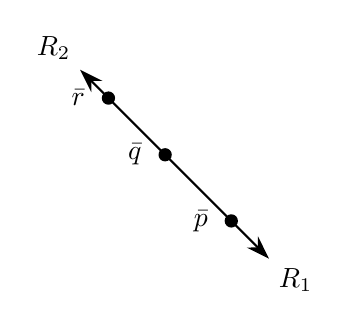
\begin{tikzpicture}[scale=0.8]
    % Define the coordinates of the endpoints
    \coordinate (R1_end) at (1, -1);
    \coordinate (R2_end) at (-2, 2);

    % Draw the arrowed line from R2 to R1
    \draw[{Stealth[length=3mm, width=2mm]}-{Stealth[length=3mm, width=2mm]}, thick] (R2_end) -- (R1_end);


    % Calculate and place points along the line using interpolation
    \path let \p1 = (R2_end), \p2 = (R1_end) in
        coordinate (r_point) at ($(\p1)!0.15!(\p2)$)
        coordinate (q_point) at ($(\p1)!0.45!(\p2)$)
        coordinate (p_point) at ($(\p1)!0.8!(\p2)$);

    % Draw the points
    \fill (r_point) circle (3pt) node[left=5pt] {$\bar{r}$};
    \fill (q_point) circle (3pt) node[left=5pt] {$\bar{q}$};
    \fill (p_point) circle (3pt) node[left=5pt] {$\bar{p}$};

    % Label the endpoints
    \node[below right] at (R1_end) {$R_1$};
    \node[above left] at (R2_end) {$R_2$};
\end{tikzpicture}
\end{center}

  \item If $\bar{x} \in L$, then $\bar{x} \in R_1$ if and only if $\bar{x}$ is on the line segment between $\bar{p}$ and $\bar{q}$, or
        $\bar{p}$ is between $\bar{q}$ and $\bar{x}$. We therefore refer to $R_1$ as the ray with origin $\bar{q}$ in the direction of
        $\bar{p}$, and call $(\bar{p} - \bar{q})$ the direction vector of $R_1$.

        \begin{center}
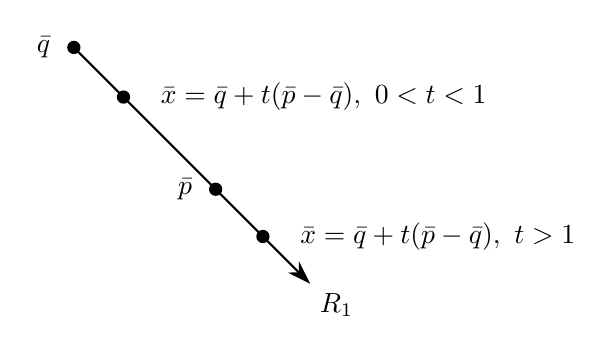
\begin{tikzpicture}[scale=1.2]

  % Define endpoints
  \coordinate (R1) at (2.5, -2.5);
  \coordinate (Q)  at (0, 0);

  % Draw the line with arrow from q to R1
  \draw[-{Stealth[length=3mm, width=2mm]}, thick] (Q) -- (R1);

  % Point p in between q and R1
  \path let \p1 = (Q), \p2 = (R1) in
    coordinate (P) at ($(\p1)!0.6!(\p2)$);

  % Mark points
  \fill (Q) circle (2pt) node[left=5pt] {$\bar{q}$};
  \fill (P) circle (2pt) node[left=5pt] {$\bar{p}$};
  \node[below right] at (R1) {$R_1$};

  % Coordinates for where to place equation labels
  \path let \p1 = (Q), \p2 = (P) in
    coordinate (Eq1) at ($(\p1)!0.35!(\p2)$);

  \path let \p1 = (P), \p2 = (R1) in
    coordinate (Eq2) at ($(\p1)!0.5!(\p2)$);

  % Draw closed dots at the equation positions
  \fill (Eq1) circle (2pt);
  \fill (Eq2) circle (2pt);

  % Add equations
  \node[right=10pt] at (Eq1) 
    {$\bar{x} = \bar{q} + t(\bar{p} - \bar{q}),\ 0 < t < 1$};

  \node[right=10pt] at (Eq2) 
    {$\bar{x} = \bar{q} + t(\bar{p} - \bar{q}),\ t > 1$};

\end{tikzpicture}
\end{center}

        
  \item For any two points $\bar{p}$ and $\bar{q}$ in $\mathbb{R}^3$, the set $R = \{\bar{q}+t\bar{p} : t \geq 0\}$ is a ray. Indeed,
  
  \[R=\{\bar{q}+t([\bar{p}+\bar{q}] - \bar{q}) : t \geq 0\}.\]
  Therefore $R$ is the ray with origin $\bar{q}$ in the direction of $\bar{p}+\bar{q}$.
  
  \end{enumerate}
\end{remarkbox}

\newpage
The following table shows how the concepts of lines, rays, line segments and betweenness
 are related to one another.
\begin{notebox}
  \[
\bar{x} = t\bar{p} + (1 - t)\bar{q}
\]

\begin{tabular}{|>{\centering\arraybackslash}m{3.5cm}
                |>{\centering\arraybackslash}m{3.5cm}
                |>{\centering\arraybackslash}m{3.5cm}
                |>{\centering\arraybackslash}m{3.5cm}|}
\hline
\textbf{Line ($t \in \mathbb{R}$)} &
\textbf{Ray ($t \geq 0$)} &
\textbf{Line segment ($0 \leq t \leq 1$)} &
\textbf{Between ($0 < t < 1$)} \\
\hline


% 1. Line
\vspace{1em}
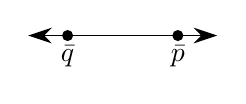
\begin{tikzpicture}
\draw[{Stealth[length=3mm, width=2mm]}-{Stealth[length=3mm, width=2mm]}] (-1.2,0) -- (1.2,0);
\fill (-0.7,0) circle (2pt) node[below] {$\bar{q}$};
\fill (0.7,0) circle (2pt) node[below] {$\bar{p}$};
\end{tikzpicture} &

% 2. Ray
\vspace{1em}
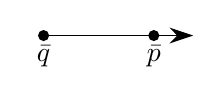
\begin{tikzpicture}
\draw[-{Stealth[length=3mm, width=2mm]}] (-0.7,0) --(1.2,0);
\fill (-0.7,0) circle (2pt) node[below] {$\bar{q}$};
\fill (0.7,0) circle (2pt) node[below] {$\bar{p}$};
\end{tikzpicture} &

% 3. Line segment
\vspace{1em}
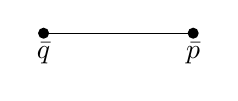
\begin{tikzpicture}
\draw[-] (-0.7,0) -- (1.2,0);
\fill (-0.7,0) circle (2pt) node[below] {$\bar{q}$};
\fill (1.2,0) circle (2pt) node[below] {$\bar{p}$};
\end{tikzpicture} &

% 4. Between
    \vspace{1em}
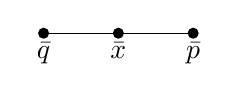
\begin{tikzpicture}
\draw[-] (-0.7,0) -- (1.2,0);
\fill (-0.7,0) circle (2pt) node[below] {$\bar{q}$};
\fill (0.25,0) circle (2pt) node[below] {$\bar{x}$};
\fill (1.2,0) circle (2pt) node[below] {$\bar{p}$};
\end{tikzpicture} \\

\hline
\end{tabular}

\end{notebox}

\begin{examplebox}

Determine whether the points 
$\bar{a} = \langle 5, -3, 6 \rangle$ and 
$\bar{b} = \langle -4, -1, -3 \rangle$ are on the line $L$ through
$\bar{p} = \langle 2, -1, 3 \rangle$ and
$\bar{q} = \langle -1, 1, 0 \rangle$.

\vspace{1em}

\textbf{Solution} 

\vspace{1em}
A point $\bar{x} \in \mathbb{R}^3$ lies on $L$ if and only if
\[
\bar{x} = \bar{q} + t(\bar{p} - \bar{q}) = \langle 3t - 1,\ 1 - 2t,\ 3t \rangle \quad \text{for some } t \in \mathbb{R}.
\]

Therefore, by the definition of vector equality, $\bar{a} = \langle 5, -3, 6 \rangle$ lies on $L$ if and only if there exists $t \in \mathbb{R}$ such that:
\[
\begin{aligned}
5 &= 3t - 1 \\
-3 &= 1 - 2t \\
6 &= 3t
\end{aligned}
\]

From the third equation, $3t = 6$ implies $t = 2$. Substituting into the first two:
\[
3(2) - 1 = 6 - 1 = 5 \quad \text{and} \quad 1 - 2(2) = 1 - 4 = -3
\]

So all three equations are satisfied with $t = 2$. Therefore, $\bar{a} \in L$.

Now consider $\bar{b} = \langle -4, -1, -3 \rangle$. This point lies on $L$ if there exists $t \in \mathbb{R}$ such that:
\[
\begin{aligned}
-4 &= 3t - 1 \\
-1 &= 1 - 2t \\
-3 &= 3t
\end{aligned}
\]

From the third equation, $3t = -3$ implies $t = -1$. Substituting into the second equation:
\[
1 - 2(-1) = 1 + 2 = 3 \ne -1
\]

So $t = -1$ satisfies the third equation but not the second. Hence, no single $t$ satisfies all three equations. Therefore, $\bar{b} \notin L$.

\end{examplebox}
\begin{examplebox}
Determine whether or not the points \(\bar{b} = \langle 0, 3, 0 \rangle\) and \(\bar{c} = \left\langle \frac{3}{2}, 0, \frac{3}{2} \right\rangle\) are on the line segment \(S\) between the points \(\bar{p} = \langle 1, 1, 1 \rangle\) and \(\bar{q} = \langle 2, -1, 2 \rangle\).
\vspace{1em}

\textbf{Solution} 
\vspace{1em}

For a point \(\bar{x}\), we have
\[
\bar{x} \in S \iff \bar{x} = t\bar{p} + (1 - t)\bar{q} \quad \text{for some } 0 \leq t \leq 1.
\]

Hence, the point \(\bar{b} = \langle 0, 3, 0 \rangle\) is on the line segment \(S\) if and only if there exists a real number \(0 \leq t \leq 1\) such that
\[
\bar{b} = t\bar{p} + (1 - t)\bar{q} = \langle 2 - t, 2t - 1, 2 - t \rangle.
\]

So \(\bar{b} \in S\) if and only if the following equations are satisfied:
\[
0 = 2 - t, \quad 3 = 2t - 1, \quad 0 = 2 - t.
\]

From the first equation, we get \(t = 2\). This value of \(t\) also satisfies the second and third equations, so:
\[
\bar{b} = 2\bar{p} + (1 - 2)\bar{q}.
\]

Therefore, \(\bar{b}\) is on the line through \(\bar{p}\) and \(\bar{q}\). However, \(t = 2 > 1\), so \(\bar{b}\) is not on the line segment \(S\) between \(\bar{p}\) and \(\bar{q}\).

Now consider the point \(\bar{c} = \left\langle \frac{3}{2}, 0, \frac{3}{2} \right\rangle\). This point is on \(S\) if and only if
\[
\bar{c} = t\bar{p} + (1 - t)\bar{q} = \langle 2 - t, 2t - 1, 2 - t \rangle \quad \text{for some } 0 \leq t \leq 1.
\]

Thus, \(\bar{c} \in S\) if and only if
\[
\frac{3}{2} = 2 - t, \quad 0 = 2t - 1, \quad \frac{3}{2} = 2 - t.
\]

The first equation implies \(t = \frac{1}{2}\). This value also satisfies the other equations. Therefore,
\[
\bar{c} = \frac{1}{2} \bar{p} + \left(1 - \frac{1}{2}\right) \bar{q}.
\]

Since \(0 \leq \frac{1}{2} \leq 1\), it follows that \(\bar{c} \in S\).
\end{examplebox}

In the following examples we investigate the intersection of lines in space
$L_1 = \left\{ \bar{q} + t(\bar{p} - \bar{q}) : t \in \mathbb{R} \right\}$ and $L_2 = \left\{ \bar{b} + s(\bar{a} - \bar{b}) : s \in \mathbb{R} \right\}$
in space intersect at a point \(\bar{x}\) if and only if \(\bar{x} \in L_1 \cap L_2\). That is, the lines intersect at \(\bar{x}\) if and only if both
$\bar{x} = \bar{q} + t(\bar{p} - \bar{q})$ for some $t \in \mathbb{R}$ and $\bar{x} = \bar{b} + s(\bar{a} - \bar{b})$ for some  $s \in \mathbb{R}.$

Note that it is possible for \(L_1\) and \(L_2\) to:
\begin{itemize}
  \item intersect at exactly one point,
  \item not intersect at all (e.g., parallel lines), or
  \item intersect at infinitely many points (if they coincide).
\end{itemize}
\begin{examplebox}
Consider the line \(L_1\) through \(\bar{p} = \langle 1, 0, 1 \rangle\) and \(\bar{q} = \langle 0, 2, 0 \rangle\), and the line \(L_2\) through the points \(\bar{a} = \langle 2, 1, 2 \rangle\) and \(\bar{b} = \langle 0, 3, 0 \rangle\). 

Determine whether or not \(L_1\) and \(L_2\) intersect, and find all points of intersection, if any exist.

\vspace{1em}

\textbf{Solution}

\vspace{1em}

The lines \(L_1\) and \(L_2\) intersect at a point \(\bar{x} = \langle x, y, z \rangle\) if and only if \(\bar{x} \in L_1\) and \(\bar{x} \in L_2\). Therefore, \(L_1\) and \(L_2\) intersect at \(\bar{x}\) if and only if
\[
\bar{q} + t(\bar{p} - \bar{q}) = \bar{x} = \bar{b} + s(\bar{a} - \bar{b}) \quad \text{for some } t, s \in \mathbb{R}. \tag{i}
\]

It then follows from the definition of vector equality that
\[
t = x = 2s, \qquad 2 - 2t = y = 3 - 2s, \qquad t = z = 2s.
\]

The third equation implies that \(t = 2s\). Substituting \(t = 2s\) into the second equation yields:
\[
2 - 2(2s) = 3 - 2s \quad \Rightarrow \quad -2s = 1 - 2s \quad \Rightarrow \quad s = -\frac{1}{2}.
\]

Hence \(t = 2s = -1\). These values for \(s\) and \(t\) also satisfy the first equation, since
\[
t = -1 = 2\left(-\frac{1}{2}\right) = 2s.
\]

Therefore, these are the only values for \(t\) and \(s\) that satisfy (i). Thus, \(L_1\) and \(L_2\) intersect at the single point
\[
\bar{x} = \bar{q} - (\bar{p} - \bar{q}) = \langle -1, 4, -1 \rangle.
\]
\end{examplebox}

\begin{examplebox}
Determine whether or not the lines \(L_1 = \{ \langle 1 - t, 1 - t, 2t \rangle : t \in \mathbb{R} \}\) and 

\(L_2 = \{ \langle s, 2, s - 1 \rangle : s \in \mathbb{R} \}\) intersect, and find the points of intersection, if any exist.

\vspace{0.5em}

\textbf{Solution}

\vspace{0.5em}

The lines \(L_1\) and \(L_2\) intersect at a point \(\bar{x} = \langle x, y, z \rangle\) if and only if \(\bar{x} \in L_1\) and \(\bar{x} \in L_2\). Therefore, \(L_1\) and \(L_2\) intersect at \(\bar{x}\) if and only if
\[
\langle 1 - t, 1 - t, 2t \rangle = \bar{x} = \langle s, 2, s - 1 \rangle \quad \text{for some } t, s \in \mathbb{R}. \tag{i}
\]

From the definition of vector equality, it follows that
\[
1 - t = x = s, \qquad 1 - t = y = 2, \qquad 2t = z = s - 1.
\]

The second equation implies that \(t = -1\). Substituting \(t = -1\) into the first equation gives:
\[
s = 1 - (-1) = 2.
\]

Substituting \(t = -1\) into the third equation yields:
\[
2(-1) = -2 = s - 1 \quad \Rightarrow \quad s = -1.
\]

Since \(2 \neq -1\), it follows that there are no real numbers \(t\) and \(s\) that satisfy (i). Therefore, the lines \(L_1\) and \(L_2\) do not intersect.
\end{examplebox}

\begin{examplebox}
  Let $L_1$ be the line with equation $\bar{x} = \langle 1 + t,\, 2 + t,\, 3 + t \rangle,\text{ } t \in \mathbb{R},$
and $L_2$ the line with equation $\bar{x} = \langle 2 - 2s,\, 3 - 2s,\, 4 - 2s \rangle, \text{ } s \in \mathbb{R}.$

Determine whether or not these lines intersect, and find the points of intersection, if any such points exist.

\vspace{0.5em}

\textbf{Solution}

\vspace{0.5em}

The lines $L_1$ and $L_2$ intersect at a point $\bar{x} = \langle x, y, z \rangle$ if and only if $\bar{x} \in L_1$ and $\bar{x} \in L_2$. Therefore, $L_1$ and $L_2$ intersect at $\bar{x}$ if and only if
\[
\langle 1 + t,\, 2 + t,\, 3 + t \rangle = \bar{x} = \langle 2 - 2s,\, 3 - 2s,\, 4 - 2s \rangle
\]
for some $t, s \in \mathbb{R}$.

It follows from the definition of vector equality that
\[
1 + t = x = 2 - 2s, \quad 2 + t = y = 3 - 2s, \quad 3 + t = z = 4 - 2s.
\tag{A}
\]

All three equations imply that $t = 1 - 2s.$ Hence for every real number $s$, there exists a real number $t = 1 - 2s$ such that $t$ and $s$ satisfy (A). 

Therefore, if 
$\bar{x} = \langle 2 - 2s,\, 3 - 2s,\, 4 - 2s \rangle \in L_2,$
then
$\bar{x} = \langle 1 + (1 - 2s),\, 2 + (1 - 2s),\, 3 + (1 - 2s) \rangle \in L_1.$

Conversely, if
$\bar{x} = \langle 1 + t,\, 2 + t,\, 3 + t \rangle \in L_1,$
then
$\bar{x} = \left\langle 2 - 2 \cdot \frac{1 - t}{2},\, 3 - 2 \cdot \frac{1 - t}{2},\, 4 - 2 \cdot \frac{1 - t}{2} \right\rangle \in L_2.$


Therefore, $L_1 = L_2$ so that every point on the line is a point of intersection.

\end{examplebox}

Our observations of the physical world tell us that, given two points $\bar{p} \neq \bar{q}$, there is exactly one straight line through $\bar{p}$ and $\bar{q}$. Another way of expressing this fact is that if two lines $L_1$ and $L_2$ intersect in more than one point, then $L_1 = L_2$. In the following theorem, we prove that this is indeed the case. This result serves as a further motivation for our definition of a line in space.

\begin{theorembox}
  
  \textbf{Equality of Lines with Multiple Intersection Points}

If two lines $L_1$ and $L_2$ intersect at more than one point, then $L_1 = L_2$.
\end{theorembox}

% LineEqualityProof.tex
% This file contains the proof

\begin{proofbox}
Let \( L_1 = \{ t\bar{p} + (1 - t)\bar{q} : t \in \mathbb{R} \} \)  
and \( L_2 = \{ s\bar{a} + (1 - s)\bar{b} : s \in \mathbb{R} \} \).  

Assume that \( L_1 \) and \( L_2 \) intersect at two distinct points, say \( \bar{u} \) and \( \bar{v} \),  
with \( \bar{u} \ne \bar{v} \). Let \( L \) be the line through \( \bar{u} \) and \( \bar{v} \).  

We shall show that \( L_1 = L = L_2 \).  

\vspace{1em}

Since \( \bar{u}, \bar{v} \in L_1 \), there exist \( t_0, t_1 \in \mathbb{R} \) such that  
\[
\bar{u} = t_0\bar{p} + (1 - t_0)\bar{q}, \quad
\bar{v} = t_1\bar{p} + (1 - t_1)\bar{q}.
\]
Since \( \bar{u} \ne \bar{v} \), it follows that \( t_0 \ne t_1 \).  

\vspace{1em}

Now consider a point
\[
\bar{x} = r(t_0\bar{p} + (1 - t_0)\bar{q}) + (1 - r)(t_1\bar{p} + (1 - t_1)\bar{q}).
\]
By the properties of vector addition and scalar multiplication,
\begin{align*}
\bar{x}
&= \big( rt_0 + (1 - r)t_1 \big) \bar{p}
+ \big( r(1 - t_0) + (1 - r)(1 - t_1) \big) \bar{q} \\
&= \big( rt_0 + t_1 - rt_1 \big) \bar{p}
+ \big( r - rt_0 + 1 - r - (1 - t_1) \big) \bar{q} \\
&= \big( rt_0 + t_1 - rt_1 \big) \bar{p}
+ \big( 1 - (rt_0 + t_1 - rt_1) \big) \bar{q}.
\end{align*}
Hence \( \bar{x} \in L_1 \). But \( \bar{x} \) was a point on the line through \( \bar{u} \) and \( \bar{v} \),  
so this shows every point on the line \( L \) lies in \( L_1 \).  

\vspace{1em}

Now, using the identities:
\[
\bar{u} = t_0\bar{p} + (1 - t_0)\bar{q}, \quad
\bar{v} = t_1\bar{p} + (1 - t_1)\bar{q},
\]
we multiply both by \( t_1 \) and \( t_0 \), respectively:
\begin{align*}
t_1\bar{u} &= t_1t_0\bar{p} + t_1(1 - t_0)\bar{q} \tag{A} \\
t_0\bar{v} &= t_0t_1\bar{p} + t_0(1 - t_1)\bar{q} \tag{B}
\end{align*}


\end{proofbox}
\begin{proofbox}
Subtracting (B) from (A):
\begin{align*}
t_1\bar{u} - t_0\bar{v}
&= t_1(1 - t_0)\bar{q} - t_0(1 - t_1)\bar{q} \\
&= \big( t_1 - t_0 \big)\bar{q} \\
\Rightarrow \quad \bar{q} &= \frac{t_1\bar{u} - t_0\bar{v}}{t_1 - t_0}
= \frac{t_0}{t_1 - t_0} \bar{u} - \frac{t_1}{t_1 - t_0} \bar{v} \tag{C}
\end{align*}

\vspace{1em}


Likewise, observe:
\begin{align*}
\bar{u} - \bar{v}
&= (t_0 - t_1)\bar{p} + (1 - t_0 - (1 - t_1))\bar{q} \\
&= (t_0 - t_1)\bar{p} + (t_1 - t_0)\bar{q} \\
&= (t_0 - t_1)(\bar{p} - \bar{q}) \\
\Rightarrow \quad \bar{p}
&= \frac{1 - t_0}{t_0 - t_1} \bar{u} - \frac{1 - t_1}{t_0 - t_1} \bar{v} \tag{D}
\end{align*}
    
Now suppose that \( \bar{y} \in L_1 \). Then \( \bar{y} = t\bar{p} + (1 - t)\bar{q} \) for some \( t \in \mathbb{R} \).  
Substitute from (C) and (D):
\begin{align*}
\bar{y}
&= t\left( \frac{1 - t_0}{t_0 - t_1} \bar{u} - \frac{1 - t_1}{t_0 - t_1} \bar{v} \right)
+ (1 - t) \left( \frac{t_0}{t_1 - t_0} \bar{u} - \frac{t_1}{t_1 - t_0} \bar{v} \right) \\
&= \left( \frac{t(1 - t_0)}{t_0 - t_1} + \frac{(1 - t)t_0}{t_0 - t_1} \right) \bar{u}
+ \left( -\frac{t(1 - t_1)}{t_0 - t_1} - \frac{(1 - t)t_1}{t_0 - t_1} \right) \bar{v} \\
&= \frac{t - t_1}{t_0 - t_1} \bar{u}
+ \left( 1 - \frac{t - t_1}{t_0 - t_1} \right) \bar{v}.
\end{align*}

Thus \( \bar{y} \in L \). So every point on \( L_1 \) lies on \( L \), i.e., \( L_1 \subseteq L \).  
By symmetry, the same argument shows \( L_2 \subseteq L \).  
Hence, \( L_1 = L = L_2 \).  
\hfill \( \qed \)
\end{proofbox}


\vspace{1em}
  As with parallel lines in coordinate geometry, we can also define parallel lines in our model for space:
  \begin{definitionbox}
    \textbf{Parallel Lines in Space}

    Two lines $L_1 = \{\bar{q} +t(\bar{p} - \bar{q}) : t \in \mathbb{R}\}$ and $L_2 = \{\bar{b} +t(\bar{a} - \bar{b}) : t \in \mathbb{R}\}$ are \textit{parallel} if and only if

    \[
      \bar{p}-\bar{q} = k(\bar{a}-\bar{b}) \text{ for some } k \in \mathbb{R} \text{ such that } k \neq 0.
    \]

  \end{definitionbox}

\begin{remarkbox}
 Consider the lines $L_1 = \{ \bar{q} + t(\bar{p} - \bar{q}) : t \in \mathbb{R} \}$ and $L_2 = \{ \bar{b} + t(\bar{a} - \bar{b}) : t \in \mathbb{R} \}$
in $ \mathbb{R}^3$.

If \( \alpha \) is a non-zero real number, then
\[
\bar{p} - \bar{q} = \alpha (\bar{a} - \bar{b}) \quad \text{if and only if} \quad
\bar{a} - \bar{b} = \frac{1}{\alpha}(\bar{p} - \bar{q}).
\]

Therefore, \( L_1 \) and \( L_2 \) are \textbf{parallel} if and only if
\[
\bar{a} - \bar{b} = \beta (\bar{p} - \bar{q}) \quad \text{for some non-zero real number } \beta.
\]

This essentially means that one vector is a scalar multiple of the other. Geometrically, the lines are parallel if they go in the same direction (or exactly opposite).
\end{remarkbox}
\vspace{1em}
Intuitively, if two distinct lines \( L_1 \) and \( L_2 \) are parallel, then \( L_1 \) and \( L_2 \) do not intersect.
In terms of our model of space, we can prove this idea, all while motivating our definition of parallel lines, with the following theorem:

\begin{theorembox}
  \textbf{Non-Intersection of Parallel Lines}

  If $L_1$ and $L_2$ are distinct parallel lines in $\mathbb{R}^3$, then they do not intersect.
\end{theorembox}

\begin{proofbox}
Let \( L_1 = \{ \bar{q} + t(\bar{p} - \bar{q}) : t \in \mathbb{R} \} \) and  
\( L_2 = \{ \bar{b} + s(\bar{a} - \bar{b}) : s \in \mathbb{R} \} \) be distinct parallel lines in \( \mathbb{R}^3 \). Since \( L_1 \neq L_2 \), and the lines are parallel, they do not coincide.  
Thus, we may assume (without loss of generality) that \( \bar{q} \notin L_2 \), i.e., $\bar{q} \neq \bar{b} + s(\bar{a} - \bar{b}) \text{ for all } s \in \mathbb{R}.$

\vspace{0.5em}

Since \( L_1 \) and \( L_2 \) are parallel, there exists a non-zero real number \( \alpha \) such that 

$\bar{p} - \bar{q} = \alpha(\bar{a} - \bar{b}).$
Therefore, it follows that $L_1 = \{ \bar{q} + \alpha t(\bar{a} - \bar{b}) : t \in \mathbb{R} \}$.

\vspace{0.5em}

Now suppose, for contradiction, that \( L_1 \) and \( L_2 \) intersect at some point \( \bar{x} \in \mathbb{R}^3 \).  
Then there exist \( t_0, s_0 \in \mathbb{R} \) that satisfy: 

$\bar{x} = \bar{q} + \alpha t_0 (\bar{a} - \bar{b}) = \bar{b} + s_0 (\bar{a} - \bar{b})$.

Subtracting \( \alpha t_0 (\bar{a} - \bar{b}) \) from both sides yields

\(\bar{q} = \bar{b} + s_0 (\bar{a} - \bar{b}) - \alpha t_0 (\bar{a} - \bar{b}) \\
\quad = \bar{b} + (s_0 - \alpha t_0)(\bar{a} - \bar{b}).
\)

\vspace{0.5em}
Now let \( s = s_0 - \alpha t_0 \). Then
\(
\bar{q} = \bar{b} + s(\bar{a} - \bar{b}),
\)
which implies \( \bar{q} \in L_2 \), evidently contradicting our earlier assumption that \( \bar{q} \notin L_2 \).
 
Hence, \( L_1 \) and \( L_2 \) do not intersect.

\hfill $\qed$
\end{proofbox}

\begin{notebox}
  The Theorem of Non-Intersection of Parallel Lines states that distinct parallel lines do not intersect.
  The converse of this theorem, however, is generally false. If two lines $L_1$ and $L_2$ do not intersect, it does not follow that they are parallel.
\end{notebox}
\begin{examplebox}
Let \( L_1 \) be the line through \( \bar{p} = \langle 2, 3, 1 \rangle \) and \( \bar{q} = \langle 4, 5, 5 \rangle \), and \( L_2 \) the line through \( \bar{a} = \langle -1, 1, 2 \rangle \) and \( \bar{b} = \langle 5, 7, 14 \rangle \). Determine whether or not \( L_1 \) and \( L_2 \) are parallel.

\vspace{0.5em}

\textbf{Solution}

\vspace{0.5em}

\( \bar{p} - \bar{q} = \langle -2, -2, -4 \rangle \) and \( \bar{a} - \bar{b} = \langle 6, 6, 12 \rangle \).  
Therefore  
\( \bar{a} - \bar{b} = \langle 6, 6, 12 \rangle = -3\langle -2, -2, -4 \rangle = -3(\bar{p} - \bar{q}) \).  
Therefore \( L_1 \) and \( L_2 \) are parallel.
\end{examplebox}

\begin{examplebox}
Let \( L_1 = \{\langle 1 - t, 1 - t, 2t \rangle : t \in \mathbb{R} \} \) and \( L_2 = \{\langle s, 2, s - 1 \rangle : s \in \mathbb{R} \} \).  
Given that \( L_1 \) and \( L_2 \) do not intersect, show that \( L_1 \) and \( L_2 \) are not parallel.

\vspace{0.5em}

\textbf{Solution}

\vspace{0.5em}

By the definition of vector addition, and scalar multiplication, \( L_1 \) and \( L_2 \) can be expressed as  
\[
L_1 = \{\langle 1, 1, 0 \rangle + t\langle -1, -1, 2 \rangle : t \in \mathbb{R} \}
\]
and  
\[
L_2 = \{\langle 0, 2, -1 \rangle + s\langle 1, 0, 1 \rangle : s \in \mathbb{R} \}.
\]

If \( L_1 \) and \( L_2 \) were parallel, then  
\(
\langle -1, -1, 2 \rangle = \alpha \langle 1, 0, 1 \rangle = \langle \alpha, 0, \alpha \rangle
\)
for some \( \alpha \in \mathbb{R} \).  
By the definition of vector equality, it is implied that \( -1 = 0 \), which is not true.  
Therefore \( L_1 \) and \( L_2 \) are not parallel.
\end{examplebox}

\begin{examplebox}
  Consider the points \(\bar{p} = \langle 1, 0, 2 \rangle\), \(\bar{q} = \langle c, 2, 1 \rangle\), \(\bar{a} = \langle 5, c, 3 \rangle\), and \(\bar{b} = \langle -7, -1, 1 \rangle\) in \(\mathbb{R}^3\), where \(c \in \mathbb{R}\) is a constant. We determine all values of \(c\), if any, so that the line through \(\bar{p}\) and \(\bar{q}\) is parallel to the line through \(\bar{a}\) and \(\bar{b}\).

\vspace{1em}

\textbf{Solution}

\vspace{1em}

By definition, the line through \(\bar{p}\) and \(\bar{q}\) is parallel to the line through \(\bar{a}\) and \(\bar{b}\) if and only if there exists a non-zero real number \(\alpha\) such that
\(
\bar{a} - \bar{b} = \alpha (\bar{p} - \bar{q}).
\)

We have
\(
\bar{a} - \bar{b} = \langle 12, c + 1, 2 \rangle \text{ and } \bar{p} - \bar{q} = \langle 1 - c, -2, 1 \rangle.
\)

Therefore, for a real number \(\alpha\), the equation \(\bar{a} - \bar{b} = \alpha (\bar{p} - \bar{q})\) holds if and only if
\[
12 = \alpha (1 - c), \quad c + 1 = -2\alpha, \quad \alpha = 2.
\]

According to the last equation, if \(\bar{a} - \bar{b} = \alpha (\bar{p} - \bar{q})\), then \(\alpha = 2\). Substituting \(\alpha = 2\) into the first and second equations yields
\[
12 = 2 (1 - c) \quad \text{and} \quad c + 1 = -4.
\]

Both equations imply that \(c = -5\). Therefore, the line through \(\bar{p}\) and \(\bar{q}\) is parallel to the line through \(\bar{a}\) and \(\bar{b}\) if and only if \(c = -5\).

\end{examplebox}

\vspace{1em}

Now beyond lines in space, our model for space even holds for three-dimensional objects! One such object that appears frequently in applications is the sphere.
Consider the fact that the Earth and other celestial bodies are approximated as spheres. As we have done before, we define a sphere in terms of our model for space.

\begin{definitionbox}

  \textbf{Sphere}

  Let \(\bar{c}\) be a point in \(\mathbb{R}^3\), and let \(r > 0\) be a real number.  
The sphere with center \(\bar{c}\) and radius \(r\) is the set
\[
S = \{\bar{x} \in \mathbb{R}^3 : \|\bar{c} - \bar{x}\| = r \}.
\]
\end{definitionbox}

Consider a sphere
\[
S = \{\bar{x} \in \mathbb{R}^3 : \|\bar{c} - \bar{x}\| = r\}.
\]
The set \(S\) consists of all points in space that are at a distance \(r\) from the fixed point \(\bar{c}\), the center of the sphere. The sphere \(S\) is shown in the figure below.


\begin{center}
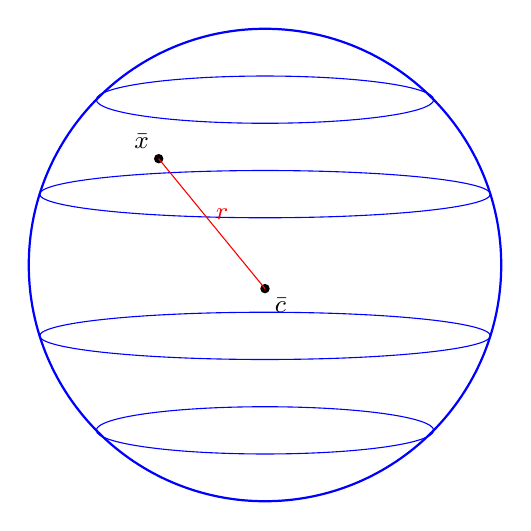
\begin{tikzpicture}[scale=3]
    

  % Outer Sphere
  \shade[ball color=white, opacity=0.0] (0,0) circle(1); % invisible shading
  \draw[blue, thick] (0,0) circle(1); % sphere boundary

  % Latitude lines (ellipses)
  \foreach \y in {-0.7,-0.3,0.3,0.7}
    \draw[blue, thin] (0,\y) ellipse ({sqrt(1 - \y*\y)} and 0.1);

  % Points
  \coordinate (C) at (0,-0.1);
  \coordinate (X) at (-0.45,0.45);
  \fill (C) circle (0.02) node[below right] {\small$\bar{c}$};
  \fill (X) circle (0.02) node[above left] {\small$\bar{x}$};

  % Radius
  \draw[red, thin] (C) -- (X) node[midway, above right=-2pt] {\small$r$};


\end{tikzpicture}

\end{center}
Our everyday experience tells us that a line intersects a sphere in either one or two points, or not at all. Indeed, if you shoot an arrow at a soccer ball at a very high speed and do not miss, then the arrow will enter the ball at one point and exit at another, or just graze the surface of the ball. We illustrate this fact by means of some examples.

%SphereExamples.tex
%This file is part of the WTW124 course material.

\begin{examplebox}
Let $S$ be the sphere with radius $2$ and centre $\bar{0}$, and $L$ the line through the points $\bar{p} = \langle 3, 1, 0 \rangle$ and $\bar{q} = \langle 0, 0, 3 \rangle$. Determine the points where $L$ intersects $S$, if any such points exist.
\vspace{1em}

\textbf{Solution}
\vspace{1em}

$L$ intersects $S$ at a point $\bar{r}$ if and only if $\bar{r} \in S$ and $\bar{r} \in L$. Therefore $L$ intersects $S$ at $\bar{r}$ if and only if
\[
\bar{r} = t\bar{p} + (1 - t)\bar{q} = \langle 3t, t, 3 - 3t \rangle \quad \text{for some } t \in \mathbb{R}
\]
and
\[
\|\bar{r} - \bar{0}\| = 2.
\]
It is convenient to replace the last equation with
\[
\|\bar{r} - \bar{0}\|^2 = 4.
\]
Substituting the expression for $\bar{r}$ we get
\[
4 = \|\bar{r} - \bar{0}\|^2 = \| \langle 3t, t, 3 - 3t \rangle \|^2 = 9t^2 + t^2 + 9 - 18t + 9t^2.
\]
Hence
\[
19t^2 - 18t + 5 = 0.
\]
Because the discriminant of the quadratic equation satisfies
\[
\Delta = (-18)^2 - 4 \cdot 19 \cdot 5 = -56 < 0,
\]
equation has no real solutions. Therefore the line $L$ does not intersect the sphere $S$.
\end{examplebox}

\begin{examplebox}
Let $S$ be the sphere with radius $1$ and centre $\bar{c} = \langle 1, 1, 1 \rangle$, and $L$ the line through the points $\bar{p} = \langle 2, -1, 1 \rangle$ and $\bar{q} = \langle -1, 2, 1 \rangle$. Determine the points where $L$ intersects $S$, if any such points exist.
\vspace{1em}

\textbf{Solution}
\vspace{1em}

A point $\bar{r}$ lies on both $L$ and $S$ if and only if $\bar{r} \in S$ and $\bar{r} \in L$. Therefore $L$ intersects $S$ at $\bar{r}$ if and only if
\[
\bar{r} = t\bar{p} + (1 - t)\bar{q} = \langle 3t - 1, 2 - 3t, 1 \rangle \quad \text{for some } t \in \mathbb{R}
\]
and
\[
\|\bar{r} - \bar{c}\| = 1.
\]
In order to simplify our calculations, we replace this equation with
\[
\|\bar{r} - \bar{c}\|^2 = 1.
\]
Substituting, we find
\[
1 = \| \bar{r} - \bar{c} \|^2 = \| \langle 3t - 2, 1 - 3t, 0 \rangle \|^2 = 9t^2 - 12t + 4 + 1 - 6t + 9t^2.
\]
Hence
\[
18t^2 - 18t + 4 = 0.
\]
Solving, we find $t = \frac{2}{3}$ or $t = \frac{1}{3}$. Substituting these into the expression for $\bar{r}$:
\[
\bar{r}_0 = \langle 3 \cdot \tfrac{2}{3} - 1, 2 - 3 \cdot \tfrac{2}{3}, 1 \rangle = \langle 1, 0, 1 \rangle,
\]
\[
\bar{r}_1 = \langle 3 \cdot \tfrac{1}{3} - 1, 2 - 3 \cdot \tfrac{1}{3}, 1 \rangle = \langle 0, 1, 1 \rangle.
\]
\end{examplebox}

\begin{examplebox}
Let $S$ be the sphere with radius $\sqrt{2}$ and centre $\bar{c} = \langle 1, 0, 1 \rangle$, and $L$ the line through the points $\bar{p} = \langle -2, 2, 2 \rangle$ and $\bar{q} = \langle 1, -1, -1 \rangle$. Determine the points where $L$ intersects $S$, if any such points exist.
\vspace{1em}

\textbf{Solution}
\vspace{1em}

$L$ intersects $S$ at a point $\bar{r}$ if and only if $\bar{r} \in S$ and $\bar{r} \in L$. Therefore $L$ intersects $S$ at $\bar{r}$ if and only if
\[
\bar{r} = t\bar{p} + (1 - t)\bar{q} = \langle 1 - 3t, 3t - 1, 3t - 1 \rangle \quad \text{for some } t \in \mathbb{R}
\]
and
\[
\|\bar{r} - \bar{c}\| = \sqrt{2}.
\]
It is convenient to replace this with
\[
\|\bar{r} - \bar{c}\|^2 = 2.
\]
Substituting gives
\[
2 = \| \bar{r} - \bar{c} \|^2 = \| \langle -3t, 3t - 1, 3t - 2 \rangle \|^2 = 9t^2 + 9t^2 - 6t + 1 + 9t^2 - 12t + 4.
\]
Hence
\[
27t^2 - 18t + 5 = 2 \Rightarrow 9t^2 - 6t + 1 = 0.
\]
This equation has only one solution, namely $t = \frac{1}{3}$. Therefore the line $L$ intersects the sphere $S$ at precisely one point:
\[
\bar{r} = \langle 1 - 3 \cdot \tfrac{1}{3}, 3 \cdot \tfrac{1}{3} - 1, 3 \cdot \tfrac{1}{3} - 1 \rangle = \langle 0, 0, 0 \rangle = \bar{0}.
\]
\end{examplebox}


\begin{exercisebox}
1. Let $L$ be the line through $\bar{p}$ and $\bar{q}$. In each case, determine whether or not the given points $\bar{a}$ and $\bar{b}$ are on $L$. If one or both of the points is on $L$, also determine whether or not the point is between $\bar{p}$ and $\bar{q}$.
\begin{itemize}
    \item[(a)] $\bar{p} = \langle 2, 2, -3 \rangle$, $\bar{q} = \bar{0}$; $\bar{a} = \langle 1, 1, -2 \rangle$, $\bar{b} = \langle -4, -4, 6 \rangle$
    \item[(b)] $\bar{p} = \langle 1, 2, 1 \rangle$, $\bar{q} = \langle 1, 0, 2 \rangle$; $\bar{a} = \langle 1, 8, -2 \rangle$, $\bar{b} = \langle 1, 4, 1 \rangle$
    \item[(c)] $\bar{p} = \langle -1, 1, 1 \rangle$, $\bar{q} = \langle 1, 2, 2 \rangle$; $\bar{a} = \langle -5, -1, -1 \rangle$, $\bar{b} = \langle -3, 3, 3 \rangle$
    \item[(d)] $\bar{p} = \langle 2, 3, -5 \rangle$, $\bar{q} = \langle -1, 2, 1 \rangle$; $\bar{a} = \langle 5, 4, -10 \rangle$, $\bar{b} = \langle -4, 3, 7 \rangle$
    \item[(e)] $\bar{p} = \langle 0, 2, -1 \rangle$, $\bar{q} = \langle 1, 0, -1 \rangle$; $\bar{a} = \langle -4, 10, -1 \rangle$, $\bar{b} = \langle -2, 7, -1 \rangle$
\end{itemize}

2. Consider the points $\bar{p} = \langle 1, 0, 1 \rangle$ and $\bar{q} = \langle 4, 2, 6 \rangle$. Determine whether or not the points $\bar{a}, \bar{b}$ and $\bar{c}$ are between $\bar{p}$ and $\bar{q}$, where
\[
\bar{a} = \left\langle \tfrac{5}{2}, 1, \tfrac{7}{2} \right\rangle,\quad \bar{b} = \left\langle 3, \tfrac{4}{3}, \tfrac{13}{3} \right\rangle,\quad \bar{c} = \langle -2, -2, -4 \rangle.
\]

3. Determine whether or not the lines $L_1$ and $L_2$ intersect, and find the point(s) of intersection, if any exist.
\begin{itemize}
    \item[(a)] $L_1$: through $\bar{p} = \langle 1, 2, -1 \rangle$, $\bar{q} = \langle 2, 0, 1 \rangle$; 
              $L_2$: through $\bar{a} = \langle 0, 4, 1 \rangle$, $\bar{b} = \langle -2, 8, -11 \rangle$
    \item[(b)] $L_1$: through $\bar{p} = \langle -1, 0, -1 \rangle$, $\bar{q} = \langle 1, 1, 1 \rangle$; 
              $L_2$: through $\bar{a} = \langle -1, 0, -5 \rangle$, $\bar{b} = \langle 1, 1, -1 \rangle$
    \item[(c)] $L_1$: through $\bar{p} = \langle 1, 2, 1 \rangle$, $\bar{q} = \langle -1, 0, 2 \rangle$; 
              $L_2$: through $\bar{a} = \langle -2, -2, 5 \rangle$, $\bar{b} = \langle -1, -1, 6 \rangle$
    \item[(d)] $L_1$: through $\bar{p} = \langle 2, 0, -1 \rangle$, $\bar{q} = \langle 1, -2, 1 \rangle$; 
              $L_2$: through $\bar{a} = \langle 0, -4, 1 \rangle$, $\bar{b} = \langle 3, 2, -3 \rangle$
    \item[(e)] $L_1$: through $\bar{p} = \langle 2, 1, -2 \rangle$, $\bar{q} = \langle -2, -1, 2 \rangle$; 
              $L_2$: through $\bar{a} = \langle 5, 3, -6 \rangle$, $\bar{b} = \langle 1, 5, -4 \rangle$
    \item[(f)] $L_1$: through $\bar{p} = \langle 2, 3, -1 \rangle$, $\bar{q} = \langle -1, 4, 1 \rangle$; 
              $L_2$: through $\bar{a} = \langle 5, 2, -3 \rangle$, $\bar{b} = \langle -1, 4, 0 \rangle$
\end{itemize}

4. Let $\bar{c} = \langle 1, 0, 0 \rangle$ and let $S$ be the sphere with centre $\bar{c}$ and radius $2$. Determine if the line $L$ intersects the sphere $S$, and find the point(s) of intersection, if any exist.
\begin{itemize}
    \item[(a)] $L$: through $\bar{p} = \langle 1, -2, 2 \rangle$, $\bar{q} = \langle 2, -1, 1 \rangle$
    \item[(b)] $L = \{\langle 3t, 4 - 4t, 1 \rangle : t \in \mathbb{R} \}$
    \item[(c)] $L$: through $\bar{p} = \langle 0, -1, 3\sqrt{2} \rangle$, $\bar{q} = \langle 3, 2, 0 \rangle$
    \item[(d)] $L$: through $\bar{p} = \langle 3, 2\sqrt{3}, -2 \rangle$, $\bar{q} = \langle 0, -\sqrt{3}, 4 \rangle$
\end{itemize}

\end{exercisebox}

\begin{exercisebox}
    
5. Let $L$ be the line through $\bar{p} = \langle 1, 1, -1 \rangle$ and $\bar{q} = \langle -1, 2, 1 \rangle$. For the given points $\bar{a}$ and $\bar{b}$, determine the value(s) of the real number $\alpha$ so that the line through $\bar{a}$ and $\bar{b}$ intersects $L$ at exactly one point.
\begin{itemize}
    \item[(a)] $\bar{a} = \langle 1, 0, 1 \rangle$, $\bar{b} = \langle -3, 1, 3\alpha + 1 \rangle$
    \item[(b)] $\bar{a} = \langle -9, 6, \alpha^2 \rangle$, $\bar{b} = \langle 3, 0, -3 \rangle$
    \item[(c)] $\bar{a} = \langle 1, 0, 1 \rangle$, $\bar{b} = \langle -3, 1, 3\alpha + 1 \rangle$
    \item[(d)] $\bar{a} = \langle 2 + \alpha, 2, 3 \rangle$, $\bar{b} = \langle 2, 1, -1 \rangle$
\end{itemize}

6. For vectors $\bar{a}$ and $\bar{b}$ as given below, sketch the line segments between $\bar{0}$ and $\bar{a}$, $\bar{0}$ and $\bar{b}$, $\bar{a}$ and $\bar{a} + \bar{b}$, and $\bar{b}$ and $\bar{a} + \bar{b}$ in the $xy$-plane $\{ \langle x, y, 0 \rangle : x, y \in \mathbb{R} \}$. Identify the figure formed by the four line segments.
\begin{multicols}{2}
\begin{itemize}
    \item[(a)] $\bar{a} = \langle 1, 0, 0 \rangle$, $\bar{b} = \langle 0, 1, 0 \rangle$
    \item[(b)] $\bar{a} = \langle 1, 2, 0 \rangle$, $\bar{b} = \langle 2, 1, 0 \rangle$
    \item[(c)] $\bar{a} = \langle -1, 1, 0 \rangle$, $\bar{b} = \langle 2, 1, 0 \rangle$
    \item[(d)] $\bar{a} = \langle 3, 1, 0 \rangle$, $\bar{b} = \langle -2, 3, 0 \rangle$
    \item[(e)] $\bar{a} = \langle 4, 2, 0 \rangle$, $\bar{b} = \langle 2, 1, 0 \rangle$
    \item[(f)] $\bar{a} = \langle 5, 3, 0 \rangle$, $\bar{b} = \langle 2, -3, 0 \rangle$
\end{itemize}
\end{multicols}

7. Determine whether or not the given lines $L_1$ and $L_2$ are parallel.
\begin{itemize}
    \item[(a)] $L_1$: $\bar{x} = \langle 2 + 3t, -t, 2 + t \rangle$, $L_2$: $\bar{x} = \langle 1, 3, 1 \rangle + s\langle 6, -2, 2 \rangle$
    \item[(b)] $L_1$: through $\bar{p} = \langle -2, 1, 2 \rangle$, $\bar{q} = \langle 5, 4, -1 \rangle$; 
              $L_2$: $\bar{x} = \langle 8 - 14s, -6s, 1 + 5s \rangle$
\end{itemize}

8. Determine the value(s) of the real number $c$ for which the given lines $L_1$ and $L_2$ are parallel.
\begin{itemize}
    \item[(a)] $L_1$: $\bar{x} = \langle 4 + c^2t, -1, t + 1 \rangle$, $L_2$: $\bar{x} = \langle 4, 2, 1 \rangle + s\langle 4, 0, 2 \rangle$
    \item[(b)] $L_1$: through $\bar{p} = \langle 1, 2c, 0 \rangle$, $\bar{q} = \langle -1, 1, 1 \rangle$; 
              $L_2$: through $\bar{a} = \langle 0, 1, 1 \rangle$, $\bar{b} = \langle 1, 2, -1 \rangle$
    \item[(c)] $L_1$: through $\bar{p} = \langle c^2, 1, 1 \rangle$, $\bar{q} = \langle -1, 0, 2 \rangle$; 
              $L_2$: through $\bar{a} = \langle 3, 4, c \rangle$, $\bar{b} = \langle -1, 2, 3 \rangle$
    \item[(d)] $L_1$: $\bar{x} = \langle 1 + ct, 2, 2t + 1 \rangle$, $L_2$: $\bar{x} = \langle 2, 5, -3 \rangle + s\langle 1, 3, -1 \rangle$
    \item[(e)] $L_1$: $\bar{x} = \langle c + t, 2t - c, c - 3t \rangle$, $L_2$: $\bar{x} = \langle -2, 0, 3 \rangle + s\langle -2, -4, 6 \rangle$
\end{itemize}
\end{exercisebox}

Now that we have properly defined lines in space, we can now move onto to more specific concepts in space; in particular we will look at angles and measurements
\newpage


\subsection{Angles and Measurement}

Angles are common in the world around us: the side line and the goal line on a soccer pitch
form an angle at the point where they intersect, as do non-opposing walls in a rectangular
room. In this section we define angles in the context of our model for space, and introduce
angle measure. As a motivation for our definitions of angle and the magnitude of an angle,
we introduce triangles, and show that our definitions are consistent with the Cosine Law.

\begin{definitionbox}
\textbf{Angle}

Let \(R_1\) and \(R_2\) be two rays \(R_1 = \{\bar{a} + t\bar{p} : t \geq 0\}\) and \(R_2 = \{\bar{a} + t\bar{q} : t \geq 0\}\) with the same
origin \(\bar{a}\). The set \(R_1 \cup R_2\) of all points of all points on the two rays is called the \textbf{angle} formed by the rays \(R_1\) and \(R_2\).
\end{definitionbox}

The following figure shows the angle formed by the rays \(R_1\) and \(R_2\).

\begin{center}
    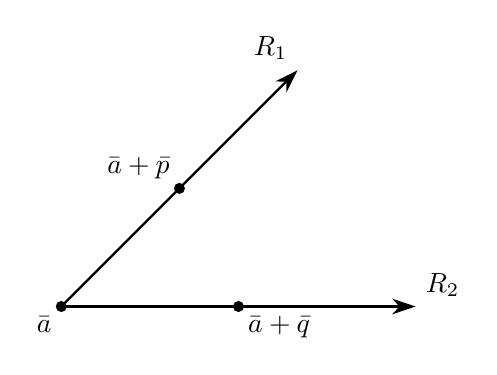
\begin{tikzpicture}
        \coordinate (R1) at (3, 3);
        \coordinate (A) at (0, 0);
        \coordinate (R2) at (4.5, 0);
        \coordinate (MdptR1) at (1.5, 1.5);
        \coordinate (MdptR2) at (2.25, 0);
 
        
        \draw[-{Stealth[length=3mm, width=2mm]}, thick] (A) -- (R1) node[above left] {$R_1$};
        \draw[-{Stealth[length=3mm, width=2mm]}, thick] (A) -- (R2) node[above right] {$R_2$};
        \fill (A) circle (2pt) node[below left] {$\bar{a}$};
        \fill (MdptR1) circle (2pt) node[above left] {$\bar{a}+\bar{p}$};
        \fill (MdptR2) circle (2pt) node[below right] {$\bar{a}+\bar{q}$};
 

    \end{tikzpicture}
\end{center}

\begin{remarkbox}
    Take note of the following regarding rays.

    \begin{enumerate}
        \item Consider two rays \(R_1 = \{\bar{a} + t\bar{p} : t \geq 0\}\) and \(R_2 = \{\bar{a} + t\bar{q} : t \geq 0\}\) with the same
origin \(\bar{a}\). If the direction vectors \(\bar{p}\) and \(\bar{q}\) are scalar multiples of each other, then \(R_1 = R_2\), or \(R_1 \cup R_2\) is a line.

        \item Let \(\bar{x}, \bar{y}, \bar{z}\) be three points not on the same line. Then the line segments \\
            \(S_1 = \{\bar{x}+t(\bar{y}-\bar{x}) : 0 \leq t \leq 1\}\) and \(S_2 = \{\bar{x}+t(\bar{z}-\bar{x}) : 0 \leq t \leq 1\}\) determine the angle formed by the rays 
            \(R_1 =\{\bar{x}+t(\bar{y}-\bar{x}): t \geq 0\}\) and \(R_2 =\{\bar{x}+t(\bar{z}-\bar{x}): t \geq 0\}\):
        \begin{center}
    \begin{tikzpicture}
        \coordinate (R1) at (3, 3);
        \coordinate (A) at (0, 0);
        \coordinate (R2) at (4.5, 0);
        \coordinate (MdptR1) at (1.5, 1.5);
        \coordinate (MdptR2) at (2.25, 0);
 
        
        \draw[-{Stealth[length=3mm, width=2mm]}, thin] (A) -- (R1) node[above left] {$R_1$};
        \draw[-{Stealth[length=3mm, width=2mm]}, thin] (A) -- (R2) node[above right] {$R_2$};
        \draw[-, very thick] (A) -- (MdptR1);
        \draw[-, very thick] (A) -- (MdptR2);
        
        \fill (A) circle (2pt) node[below left] {$\bar{x}$};
        \fill (MdptR1) circle (2pt) node[above left] {$\bar{y}$};
        \fill (MdptR2) circle (2pt) node[below right] {$\bar{z}$};
 

    \end{tikzpicture}
\end{center}  
        
    \end{enumerate}
\end{remarkbox}

\newpage

Our aim now is to define the magnitude of an angle; that is, to measure the size of an angle, 
because, in the figure below, the angle on the right is clearly `larger' than the one on the left.

\begin{center}
    
    \begin{tikzpicture}
    \coordinate (R1) at (1.5, 3);
    \coordinate (A) at (0, 0);
    \coordinate (R2) at (4.5, 0); 

    \draw[-{Stealth[length=3mm, width=2mm]}, thick] (A) -- (R1) node[above left] {$R_1$};
    \draw[-{Stealth[length=3mm, width=2mm]}, thick] (A) -- (R2) node[above right] {$R_2$};
\end{tikzpicture}
\begin{tikzpicture}
    \coordinate (R1) at (4, 3);
    \coordinate (A) at (0, 0);
    \coordinate (R2) at (4.5, 0);

    \draw[-{Stealth[length=3mm, width=2mm]}, thick] (A) -- (R1) node[above left] {$R_1$};
    \draw[-{Stealth[length=3mm, width=2mm]}, thick] (A) -- (R2) node[above right] {$R_2$};

\end{tikzpicture}

\end{center}

Now we need to quantify the what we refer to as the `size of an angle'.

\vspace{1em}

First note that for vectors \(\bar{x}, \bar{y}\), such that \(\bar{x},\bar{y} \neq 0\), by the Cauchy-Schwarz Inequality,
\(|\bar{x}\cdot \bar{y}| \leq \|\bar{x}\| \|\bar{y}\| \).

Then, by the Positive Definiteness of the Norm and the definition of the absolute value, we have

\[
    \bigg|\frac{\bar{x}\cdot \bar{y}}{\|\bar{x}\| \|\bar{y}\|}\bigg| \leq 1
\]

Finally, we find that:

\[
-1 \leq \frac{\bar{x}\cdot \bar{y}}{\|\bar{x}\| \|\bar{y}\|}\leq 1
\]

Now consider the function \(f : [0,\pi] \rightarrow \mathbb{R}\) defined by \(f(\theta)= \cos \theta\). Then \(f\) is continuous and strictly decreasing 
on the interval \([0,\pi]\), with \(f(0) = 1\) and \(f(\pi) = -1\). By the Intermediate Value Theorem, and the fact that $f$ is strictly decreasing, there exists exactly one \( \theta \in [0,\pi] \) that satisfies 

\[
    f(\theta) = \cos \theta = \frac{\bar{x}\cdot \bar{y}}{\|\bar{x}\| \|\bar{y}\|}
\]

This leads to our definition of the magnitude of an angle:

\begin{definitionbox}
\textbf{Magnitude of an Angle}

Consider the angle formed by the rays with equations \(\bar{x} = \bar{a} + t\bar{p}\) and \(\bar{x} = \bar{a} + t\bar{q}\), with \(t \geq 0\).
Then the \textit{magnitude of the angle} is the unique real number \(\theta \in [0,\pi]\) such that

\[
    \cos \theta = \frac{\bar{p}\cdot \bar{q}}{\|\bar{p}\| \|\bar{q}\|}
\]
\end{definitionbox}

\begin{remarkbox}
    Consider the angle formed by the rays \(R_1\) and \(R_2\) with equations \(\bar{x} = \bar{a} + t\bar{p}\) and \(\bar{x} = \bar{a} + t\bar{q}\), with \(t \geq 0\), respectively.
    Let \(\theta\) be the magnitude of the angle. Then

    \[
        |\bar{p}\cdot\bar{q}| = \| \bar{p}\|\cdot \| \bar{q}\| \text{ if and only if } \bar{p} \text{ and } \bar{q} \text{ are scalar multiples of each other.}
    \]

    In particular, 
    \(
        \bar{p}\cdot\bar{q} = \| \bar{p}\|\| \bar{q}\| \text{ if and only if } \bar{p} = \alpha\bar{q} \text{ for some } \alpha > 0,
    \)

    and 
    \(
        \bar{p}\cdot\bar{q} = -\| \bar{p}\|\| \bar{q}\| \text{ if and only if } \bar{p} = \alpha\bar{q} \text{ for some } \alpha < 0.
    \)

    We therefore have the following:
    \begin{enumerate}
        \item If \(\bar{p}\) and \(\bar{q}\) are not scalar multiples of each other, then \(\theta \in (0,\pi)\).
        \item If \(\bar{p} = \alpha\bar{q}\) for some \(\alpha > 0\), then \(\theta = 0\). In this case, \(R_1=R_2\), so the angle \(R_1 \cup R_2\) is a ray.
        \item If \(\bar{p} = \alpha\bar{q}\) for some \(\alpha < 0\), then \(\theta = \pi\). In this case, \(R_1 \cup R_2\) is a line.
    \end{enumerate}

\end{remarkbox}

\begin{examplebox}
Consider the rays \( R_1 \) and \( R_2 \) with equations
\(
\bar{x} = \bar{0} + t\langle 1, -1, 1 \rangle \text{ and } \bar{x} = \bar{0} + t\langle 2\alpha, 1, 1 \rangle, t \geq 0,
\)
respectively. Find all values for \( \alpha \in \mathbb{R} \) so that the angle formed by \( R_1 \) and \( R_2 \) has magnitude \( \frac{\pi}{3} \).

\vspace{0.5em}
\textbf{Solution}

\vspace{0.5em}
The direction vector for \( R_1 \) is \( \bar{p} = \langle 1, -1, 1 \rangle \), while that for \( R_2 \) is \( \bar{q} = \langle 2\alpha, 1, 1 \rangle \).

The magnitude of the angle formed by these two rays is \( \frac{\pi}{3} \) if and only if


\[
\cos\left(\frac{\pi}{3}\right) = \frac{\bar{p} \cdot \bar{q}}{\|\bar{p}\| \|\bar{q}\|} = \frac{2\alpha - 1 + 1}{\sqrt{3} \sqrt{4\alpha^2 + 2}} = \frac{2\alpha}{\sqrt{3} \sqrt{4\alpha^2 + 2}}.
\]


Since \( \cos\left(\frac{\pi}{3}\right) = \frac{1}{2} \), we equate:


\[
\frac{1}{2} = \frac{2\alpha}{\sqrt{3} \sqrt{4\alpha^2 + 2}}.
\]


Multiplying both sides by \( 2\sqrt{3} \sqrt{4\alpha^2 + 2} \), we get:


\[
\sqrt{3} \sqrt{4\alpha^2 + 2} = 4\alpha.
\]


Squaring both sides:


\[
3(4\alpha^2 + 2) = 16\alpha^2 \quad \Rightarrow \quad 12\alpha^2 + 6 = 16\alpha^2 \quad \Rightarrow \quad 4\alpha^2 = 6 \quad \Rightarrow \quad \alpha^2 = \frac{3}{2}.
\]


Thus, \( \alpha = \pm \frac{\sqrt{6}}{2} \). However, we must check which of these satisfy the original equation.

Substituting \( \alpha = \frac{\sqrt{6}}{2} \) into the original equation confirms it satisfies the condition. But \( \alpha = -\frac{\sqrt{6}}{2} \) does not, because the cosine would be negative, implying an angle greater than \( \frac{\pi}{2} \).

Therefore, the only value for \( \alpha \) for which the angle formed by the rays \( R_1 \) and \( R_2 \) is \( \frac{\pi}{3} \) is
\(
\alpha = \frac{\sqrt{6}}{2}.
\)

\end{examplebox}

\newpage

Now that we have defined angles and lines in terms of our model of space, we can define a triangle. 

\begin{definitionbox}
\textbf{Triangle}

    Let \(\bar{a}, \bar{b}, \bar{c} \in \mathbb{R}^3,\) not all on the same line. Let \(S_1\) be 
    the line segment between \(\bar{a}\) and \(\bar{b}\), \(S_2\) be the line segment between
    \(\bar{b}\) and \(\bar{c}\), and \(S_3\) be the line segment between \(\bar{a}\) and \(\bar{c}\).
    Then the \textit{triangle} with vertices \(\bar{a}\), \( \bar{b}\), and \( \bar{c}\) is the set \(S_1 \cup S_2 \cup S_3\) 
    of points on the three line segments.
\end{definitionbox}

The figure below illustrates a triangle, as defined above:

 
\begin{center}
    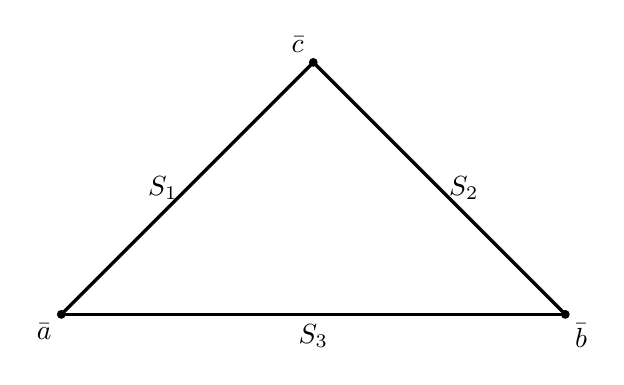
\begin{tikzpicture}[scale=0.8]
        \coordinate (A) at (-2,0);
        \coordinate (B) at (6,0);
        \coordinate (C) at (2,4);
        \coordinate (S1) at (0,2);
        \coordinate (S2) at (3,2);
        \coordinate (S3) at (0,0);

        
        \draw[very thick] (A) -- (B) node[midway, below] {};
        \draw[very thick] (B) -- (C) node[midway, right] {};
        \draw[very thick] (C) -- (A) node[midway, left] {};
        \fill (A) circle (2pt) node[below left] {$\bar{a}$};
        \fill (B) circle (2pt) node[below right] {$\bar{b}$};
        \fill (C) circle (2pt) node[above left] {$\bar{c}$};

        \node at ($(A)!0.5!(C)$) [left] {$S_1$};
        \node at ($(A)!0.5!(B)$) [below] {$S_3$};
        \node at ($(B)!0.5!(C)$) [right] {$S_2$};
        
    \end{tikzpicture}
\end{center}

\begin{remarkbox}
    Consider three points \(\bar{a}, \bar{b}, \bar{c} \in \mathbb{R}^3\), not on the same line, and the
    triangle with vertices \(\bar{a}\), \(\bar{b}\), and \(\bar{c}\).

    \begin{enumerate}
        \item The line segments \(S_1, S_2,\) and \(S_3\), joining \(\bar{a}, \bar{b},\) and \(\bar{c}\) respectively,
        are called the \textit{sides} of the triangle.
        
        \item The triangle determines three angles:
        \begin{enumerate}[label=(\alph*)]
            \item The angle at \(\bar{a}\), formed by the rays with equations 
            \(\bar{x} = \bar{a} + t(\bar{b} - \bar{a})\) and \(\bar{x} = \bar{a} + t(\bar{c} - \bar{a})\), 
            where \(t \geq 0\).
            
            \item The angle at \(\bar{b}\), formed by the rays with equations 
            \(\bar{x} = \bar{b} + t(\bar{a} - \bar{b})\) and \(\bar{x} = \bar{b} + t(\bar{c} - \bar{b})\), 
            where \(t \geq 0\).
            
            \item The angle at \(\bar{c}\), formed by the rays with equations 
            \(\bar{x} = \bar{c} + t(\bar{a} - \bar{c})\) and \(\bar{x} = \bar{c} + t(\bar{b} - \bar{c})\), 
            where \(t \geq 0\).
            The triangle with vertices \(\bar{a}\), \(\bar{b}\), and \(\bar{c}\) and the three angles
            determined by the triangle are illustrated below:
            \begin{center}
\begin{multicols}{3}
% Angle at a
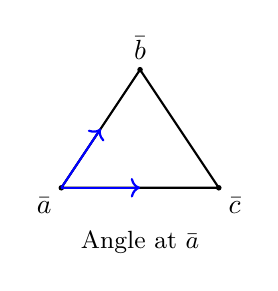
\begin{tikzpicture}[scale=0.5]
    \coordinate (A) at (0,0);
    \coordinate (B) at (2,3);
    \coordinate (C) at (4,0);

    \draw[thick] (A) -- (B) -- (C) -- cycle;

    \fill (A) circle (2pt) node[below left] {$\bar{a}$};
    \fill (B) circle (2pt) node[above] {$\bar{b}$};
    \fill (C) circle (2pt) node[below right] {$\bar{c}$};

    \draw[->, thick, color=blue] (A) -- ($(A)!0.5!(B)$);
    \draw[->, thick, color=blue] (A) -- ($(A)!0.5!(C)$);

    \node[below=5pt] at (2,-0.5) {\small Angle at $\bar{a}$};
\end{tikzpicture}

% Angle at b
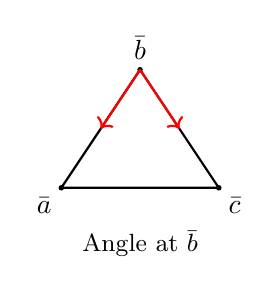
\begin{tikzpicture}[scale=0.5]
    \coordinate (A) at (0,0);
    \coordinate (B) at (2,3);
    \coordinate (C) at (4,0);

    \draw[thick] (A) -- (B) -- (C) -- cycle;

    \fill (A) circle (2pt) node[below left] {$\bar{a}$};
    \fill (B) circle (2pt) node[above] {$\bar{b}$};
    \fill (C) circle (2pt) node[below right] {$\bar{c}$};

    \draw[->, thick, color=red] (B) -- ($(B)!0.5!(A)$);
    \draw[->, thick, color=red] (B) -- ($(B)!0.5!(C)$);

    \node[below=5pt] at (2,-0.5) {\small Angle at $\bar{b}$};
\end{tikzpicture}

% Angle at c
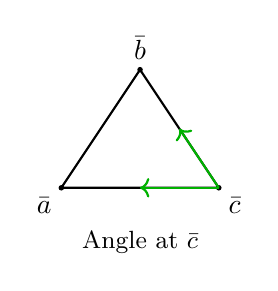
\begin{tikzpicture}[scale=0.5]
    \coordinate (A) at (0,0);
    \coordinate (B) at (2,3);
    \coordinate (C) at (4,0);

    \draw[thick] (A) -- (B) -- (C) -- cycle;

    \fill (A) circle (2pt) node[below left] {$\bar{a}$};
    \fill (B) circle (2pt) node[above] {$\bar{b}$};
    \fill (C) circle (2pt) node[below right] {$\bar{c}$};

    \draw[->, thick, color=green!70!black] (C) -- ($(C)!0.5!(A)$);
    \draw[->, thick, color=green!70!black] (C) -- ($(C)!0.5!(B)$);

    \node[below=5pt] at (2,-0.5) {\small Angle at $\bar{c}$};
\end{tikzpicture}
\end{multicols}
            \end{center}
        \end{enumerate}
    \end{enumerate}
\end{remarkbox}

\newpage

Our definition of the magnitude of an angle is consistent with the Cosine Rule.

\begin{propositionbox}
    \textbf{Cosine Rule}

    Consider a triangle with vertices \(\bar{a}\), \(\bar{b}\), and \(\bar{c}\). Let \(\theta\) be the magnitude of the angle at \(\bar{b}\). 
    \begin{center}
    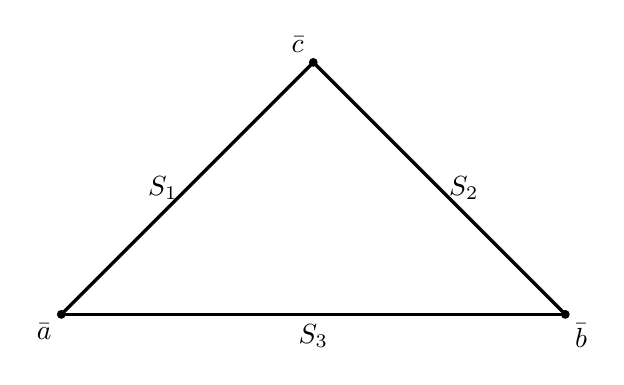
\begin{tikzpicture}[scale=0.8]
        \coordinate (A) at (-2,0);
        \coordinate (B) at (6,0);
        \coordinate (C) at (2,4);
        \coordinate (S1) at (0,2);
        \coordinate (S2) at (3,2);
        \coordinate (S3) at (0,0);

        
        \draw[very thick] (A) -- (B) node[midway, below] {};
        \draw[very thick] (B) -- (C) node[midway, right] {};
        \draw[very thick] (C) -- (A) node[midway, left] {};
        \fill (A) circle (2pt) node[below left] {$\bar{a}$};
        \fill (B) circle (2pt) node[below right] {$\bar{b}$};
        \fill (C) circle (2pt) node[above left] {$\bar{c}$};

        \node at ($(A)!0.5!(C)$) [left] {$S_1$};
        \node at ($(A)!0.5!(B)$) [below] {$S_3$};
        \node at ($(B)!0.5!(C)$) [right] {$S_2$};
        
    \end{tikzpicture}
\end{center}

    Then we have that
    
    \[
        \|\bar{a}-\bar{c}\|^2 = \|\bar{a}-\bar{b}\|^2 + \|\bar{b}-\bar{c}\|^2 - 2\|\bar{a}-\bar{b}\| \|\bar{b}-\bar{c}\| \cos \theta.
    \]    
\end{propositionbox}

\begin{proofbox}
    Calculating the square of the length of the side \(S_3\) we have:
    \[
\begin{aligned}
\|\bar{a} - \bar{c}\|^2 
&= \|(\bar{a} - \bar{b}) - (\bar{c} - \bar{b})\|^2 \\
&= \left[(\bar{a} - \bar{b}) - (\bar{c} - \bar{b})\right] \cdot \left[(\bar{a} - \bar{b}) - (\bar{c} - \bar{b})\right] \\
&= (\bar{a} - \bar{b}) \cdot (\bar{a} - \bar{b}) 
   - 2\left[(\bar{a} - \bar{b}) \cdot (\bar{c} - \bar{b})\right] 
   + (\bar{c} - \bar{b}) \cdot (\bar{c} - \bar{b}) \\
&= \|\bar{a} - \bar{b}\|^2 
   - 2\left[(\bar{a} - \bar{b}) \cdot (\bar{c} - \bar{b})\right] 
   + \|\bar{c} - \bar{b}\|^2
\end{aligned}
\]

Note that the angle at \( \bar{b} \) is determined by the rays with equations
\[
\bar{x} = \bar{b} + t(\bar{a} - \bar{b}) \quad \text{and} \quad \bar{x} = \bar{b} + t(\bar{c} - \bar{b}), \quad t \geq 0.
\]
Therefore, calculating the magnitude \( \theta \) of the angle at \( \bar{b} \), we find
\[
\cos\theta = \frac{(\bar{a} - \bar{b}) \cdot (\bar{c} - \bar{b})}{\|\bar{a} - \bar{b}\| \, \|\bar{c} - \bar{b}\|}.
\]
Hence,
\[
\|\bar{a} - \bar{c}\|^2 = \|\bar{a} - \bar{b}\|^2 + \|\bar{c} - \bar{b}\|^2 - 2\|\bar{a} - \bar{b}\| \, \|\bar{c} - \bar{b}\| \cos\theta.
\]
\end{proofbox}
\begin{examplebox}
Consider the triangle with vertices $\bar{a} = \langle 1,0,1 \rangle$, $\bar{b} = \langle 1,2,1 \rangle$, and $\bar{c} = \langle 1,2,3 \rangle$. We determine the magnitude of the angle at $\bar{a}$.

\vspace{0.5em}
\textbf{Solution.} Let $\theta$ be the magnitude of the angle at $\bar{a}$. According to the cosine rule,
\[
\|\bar{b} - \bar{c}\|^2 = \|\bar{b} - \bar{a}\|^2 + \|\bar{c} - \bar{a}\|^2 - 2\|\bar{b} - \bar{a}\|\|\bar{c} - \bar{a}\|\cos\theta.
\]
Hence,
\[
4 = 4 + 8 - 8\sqrt{2}\cos\theta \quad \Rightarrow \quad \cos\theta = \frac{1}{\sqrt{2}}.
\]
Therefore, $\theta = \frac{\pi}{4}$.
\end{examplebox}

\begin{examplebox}
Consider the triangle with vertices $\bar{a} = \langle 1,0,1 \rangle$, $\bar{b} = \langle 1,2,1 \rangle$, and $\bar{c} = \langle \alpha,1,0 \rangle$. We find the values for $\alpha$ so that the angle at $\bar{a}$ has magnitude $\frac{\pi}{3}$.

\vspace{0.5em}
\textbf{Solution.} According to the cosine rule,
\[
\|\bar{b} - \bar{c}\|^2 = \|\bar{b} - \bar{a}\|^2 + \|\bar{c} - \bar{a}\|^2 - 2\|\bar{b} - \bar{a}\|\|\bar{c} - \bar{a}\|\cos\left(\frac{\pi}{3}\right).
\]
We have:
\[
\|\bar{b} - \bar{a}\| = 2, \quad \|\bar{c} - \bar{a}\| = \sqrt{(\alpha - 1)^2 + 2}, \quad \|\bar{b} - \bar{c}\| = \sqrt{(\alpha - 1)^2 + 2}.
\]
Substituting:
\[
(\alpha - 1)^2 + 2 = 4 + (\alpha - 1)^2 + 2 - 2 \cdot 2 \cdot \sqrt{(\alpha - 1)^2 + 2} \cdot \frac{1}{2}.
\]
Simplifying:
\[
(\alpha - 1)^2 + 2 = 6 + (\alpha - 1)^2 + 2 - 2\sqrt{(\alpha - 1)^2 + 2},
\]
\[
2\sqrt{(\alpha - 1)^2 + 2} = 6 \quad \Rightarrow \quad \sqrt{(\alpha - 1)^2+2}=3 \quad \Rightarrow \quad (\alpha - 1)^2 = 7.
\]
Hence, $\alpha = 1 \pm \sqrt{7}$.
\end{examplebox}

\begin{examplebox}
Consider the triangle with vertices $\bar{a} = \langle 1,-1,1 \rangle$, $\bar{b} = \langle 2,1,1 \rangle$, and $\bar{c} = \langle -2\alpha - 1, \alpha, 6 \rangle$. We find the values for $\alpha$ so that the angle at $\bar{b}$ has magnitude $\frac{\pi}{4}$.

\vspace{0.5em}
\textbf{Solution.} Using the cosine rule:
\[
\|\bar{a} - \bar{c}\|^2 = \|\bar{a} - \bar{b}\|^2 + \|\bar{c} - \bar{b}\|^2 - 2\|\bar{a} - \bar{b}\|\|\bar{c} - \bar{b}\|\cos\left(\frac{\pi}{4}\right).
\]
We compute:
\[
\|\bar{a} - \bar{b}\| = \sqrt{5}, \quad \|\bar{a} - \bar{c}\| = \sqrt{5\alpha^2 + 10\alpha + 30}, \quad \|\bar{c} - \bar{b}\| = \sqrt{5\alpha^2 + 10\alpha + 35}.
\]
Substituting:
\[
5\alpha^2 + 10\alpha + 30 = 5 + 5\alpha^2 + 10\alpha + 35 - 2\sqrt{5}\sqrt{5\alpha^2+10\alpha+35}\cos\left(\frac{\pi}{4}\right)
\]
\[
5\alpha^2 + 10\alpha + 30 = 5\alpha^2 + 10\alpha + 40 - 2\sqrt{5}\sqrt{5\alpha^2+10\alpha+35}\frac{1}{\sqrt{2}}
\]
\[
-10 = -\sqrt{10}\sqrt{5\alpha^2+10\alpha+35} \quad \Rightarrow \quad 10 = \sqrt{10}\sqrt{5\alpha^2+10\alpha+35}
\]
\[
100 = 10(5\alpha^2+10\alpha+35) \quad \Rightarrow \quad 10=5\alpha^2+10\alpha+35 \quad \Rightarrow \quad 5\alpha^2+10\alpha+25 = 0
\]
\[
\alpha^2+2\alpha+5=0.
\]
Since the discriminant is negative, there are no real solutions. Therefore, no value of $\alpha$ gives an angle of $\frac{\pi}{4}$ at $\bar{b}$.
\end{examplebox}

\begin{examplebox}
Consider a triangle with vertices $\bar{a}$, $\bar{b}$, and $\bar{c}$ such that $\|\bar{a} - \bar{b}\| = 3$, $\|\bar{c} - \bar{a}\| = 4$, and the angle at $\bar{b}$ has magnitude $\frac{\pi}{6}$. We determine $\|\bar{b} - \bar{c}\|$.

\vspace{0.5em}
\textbf{Solution.} By the cosine rule:
\[
\|\bar{a} - \bar{c}\|^2 = \|\bar{c} - \bar{b}\|^2 + \|\bar{a} - \bar{b}\|^2 - 2\|\bar{a} - \bar{b}\|\|\bar{c} - \bar{b}\|\cos\left(\frac{\pi}{6}\right).
\]
Substituting:
\[
16 = 9 + \|\bar{b} - \bar{c}\|^2 - 2(3)\|\bar{b} - \bar{c}\|\left(\frac{\sqrt{3}}{2}\right).
\]
\[
16 = 9 + \|\bar{b} - \bar{c}\|^2 - 3\sqrt{3}\|\bar{b} - \bar{c}\|.
\]
Let $x = \|\bar{b} - \bar{c}\|$. Then:
\[
x^2 - 3\sqrt{3}x - 7 = 0.
\]
Solving using the quadratic formula:
\[
x = \frac{3\sqrt{3} \pm \sqrt{(3\sqrt{3})^2 - 4(1)(-7)}}{2} = \frac{3\sqrt{3} \pm \sqrt{27+28}}{2} = \frac{3\sqrt{3} \pm \sqrt{55}}{2}.
\]
Since $x$ must be a positive length, we take the positive root. Therefore:
\[
\|\bar{b} - \bar{c}\| = \frac{3\sqrt{3} + \sqrt{55}}{2}.
\]
\end{examplebox}
\begin{exercisebox}
\begin{enumerate}[series=AngleEX]
  \item Find the magnitude of the given angle, if it is defined. Otherwise, explain why it is not defined.
  \begin{enumerate}
    \item The angle determined by the rays with equations $\bar{x} = \bar{0} + t\langle 0, 2, 1 \rangle$ and $\bar{x} = \bar{0} + t\langle 3, -1, 2 \rangle$, $t \geq 0$
    \item The angle determined by the rays with equations $\bar{x} = \langle 1, 0, 1 \rangle + t\langle 0, 2, 0 \rangle$ and $\bar{x} = \langle 1, 0, 1 \rangle + t\langle -1, 3, \sqrt{2} \rangle$, $t \geq 0$
    \item The angle determined by the rays with equations $\bar{x} = \langle 1, 2, 3 \rangle + t\langle \sqrt{2}, -3\sqrt{2}, -2 \rangle$ and $\bar{x} = \langle 1, 2, 3 \rangle + t\langle 0, 2, 0 \rangle$, $t \geq 0$
    \item The angle determined by the rays with equations $\bar{x} = \langle -2, 2, 1 \rangle + t\langle 4, 8, 4 \rangle$ and $\bar{x} = \langle -2, 2, 1 \rangle + t\langle 1, 2, 1 \rangle$, $t \geq 0$
    \item The angle determined by the rays with equations $\bar{x} = \langle 3, 2, 1 \rangle + t\langle 1, 0, \frac{1}{\sqrt{3}} \rangle$ and $\bar{x} = \langle 2, 2, 5 \rangle + t\langle 0, 0, -1 \rangle$, $t \geq 0$
    \item The angle determined by the rays with equations $\bar{x} = \langle 2, 2, 5 \rangle + t\langle 3, 0, \sqrt{3} \rangle$ and $\bar{x} = \langle 2, 2, 5 \rangle + t\langle 0, 0, 2 \rangle$, $t \geq 0$
    \item The angle determined by the rays with equations $\bar{x} = \langle 0, -1, -3 \rangle + t\langle 1+\sqrt{3}, 2, 1 - \sqrt{\sqrt{3}} \rangle$ and $\bar{x} = \langle 0, -1, -3 \rangle + t\langle 1, 2, 1 \rangle$, $t \geq 0$
    \item The angle determined by the rays with equations $\bar{x} = \langle 0, -1, -3 \rangle + t\langle -1, 1 + 3, 2 + \sqrt{3} \rangle$ and $\bar{x} = \langle 0, -1, -3 \rangle + t\langle -2, -4, -2 \rangle$, $t \geq 0$
    \item The angle determined by the rays with equations $\bar{x} = \langle 1, 2, 1 \rangle + t\langle 1, 1, 2 \rangle$ and $\bar{x} = \langle 1, 2, 1 \rangle + t\langle -1, -1, 2 \rangle$, $t \geq 0$
  \end{enumerate}

  \item Consider the triangle with vertices $\bar{a}, \bar{b}, \bar{c}$. In each case, find the magnitude of the specified angle.
  \begin{enumerate}
    \item $\bar{a} = \langle 1,1,1 \rangle$, $\bar{b} = \langle 1,3,2 \rangle$, $\bar{c}= \langle 7,-1,5 \rangle$; the angle at $\bar{a}$
    \item $\bar{a} = \langle 1,-1,1 \rangle$, $\bar{b} = \langle 1,3,1 \rangle$, $\bar{c}= \langle 1 - \sqrt{2}, 3\sqrt{2} - 1, 3 \rangle$; the angle at $\bar{a}$
    \item $\bar{a} = \langle 1,1,1 \rangle$, $\bar{b} = \langle 0,1,0 \rangle$, $\bar{c}= \langle 0,0,1 \rangle$; the angle at $\bar{c}$
    \item $\bar{a} = \bar{0}$, $\bar{b} = \langle 2, -6, -2\sqrt{2} \rangle$, $\bar{c}= \langle 0, 1, 0 \rangle$; the angle at $\bar{a}$
    \item $\bar{a} = \langle \sqrt{3}, 3, -\sqrt{3} \rangle$, $\bar{b} = \langle 1, 5, 1 \rangle$, $\bar{c} = \langle -1, 1, -1 \rangle$; the angle at $\bar{c}$
    \item $\bar{a} = \langle 0, 2, -3 \rangle$, $\bar{b} = \langle \sqrt{3}, 2, -2 \rangle$, $\bar{c}= \langle 0, 2, -5 \rangle$; the angle at $\bar{a}$
    \item $\bar{a} = \langle 2, 1, 3\sqrt{3} \rangle$, $\bar{b} = \langle -1, 1, 2\sqrt{3} \rangle$, $\bar{c}= \langle -1, 1, 4\sqrt{3} \rangle$; the angle at $\bar{b}$
  \end{enumerate}

  \item Consider the triangle with vertices $\bar{a} = \bar{0}$, $\bar{b} = \langle 1, 2, 1 \rangle$, and $\bar{c} = \langle 0, \alpha, 1 \rangle$. Find the values of $\alpha$ such that the magnitude of the angle at $\bar{a}$ is:
  \begin{multicols}{2}
  \begin{enumerate}
    \item $\frac{\pi}{6}$
    \item $\frac{\pi}{4}$
    \item $\frac{\pi}{3}$
    \item $\arccos\left( \frac{2\sqrt{2}}{\sqrt{3}} \right)$
    \item $\frac{5\pi}{6}$
    \item $\frac{3\pi}{4}$
    \item $\frac{\pi}{2}$
  \end{enumerate}
  \end{multicols}
  \end{enumerate}
\end{exercisebox}

\begin{exercisebox}
  \begin{enumerate}[resume=AngleEX]  

  \item Consider a triangle with vertices $\bar{a}, \bar{b}, \bar{c}$. Determine the following:
  \begin{enumerate}
    \item $\|\bar{a} - \bar{c}\|$ if $\|\bar{a} - \bar{b}\| = 2$, $\|\bar{c} - \bar{b}\| = 3$, and the angle at $\bar{b}$ has magnitude $\frac{\pi}{6}$.
    \item $\|\bar{a} - \bar{b}\|$ if $\|\bar{a} - \bar{c}\| = 2$, $\|\bar{c} - \bar{b}\| = 3$, and the angle at $\bar{b}$ has magnitude $\frac{\pi}{3}$.
    \item $\|\bar{a} - \bar{b}\|$ if $\|\bar{a} - \bar{c}\| = 3$, $\|\bar{c} - \bar{b}\| = 2$, and the angle at $\bar{b}$ has magnitude $\frac{\pi}{2}$.
    \item $\|\bar{a} - \bar{b}\|$ if $\|\bar{a} - \bar{c}\| = 3$, the angle at $\bar{a}$ is $\frac{\pi}{3}$ and the angle at $\bar{c}$ is $\frac{\pi}{2}$.
  \end{enumerate}

  \item Let $\bar{a}, \bar{b}, \bar{c}$ be the vertices of a triangle. Show that if the angle at $\bar{a}$ has magnitude $\frac{\pi}{2}$, then $\|\bar{b} - \bar{c}\|^2 = \|\bar{a} - \bar{c}\|^2 + \|\bar{a} - \bar{b}\|^2$.

  \item Let $\bar{a}, \bar{b}, \bar{c}$ be the vertices of a triangle. Show that if $\|\bar{b} - \bar{c}\|^2 = \|\bar{a} - \bar{c}\|^2 + \|\bar{a} - \bar{b}\|^2$, then the angle at $\bar{a}$ has magnitude $\frac{\pi}{2}$.

  \item Let $\bar{a}, \bar{b}, \bar{c}$ be the vertices of a triangle. If the angles at $\bar{a}$ and $\bar{c}$ have the same magnitude, show that $\|\bar{b} - \bar{a}\| = \|\bar{b} - \bar{c}\|$.

  \item Let $\bar{a}, \bar{b}, \bar{c}$ be the vertices of a triangle. If $\|\bar{b} - \bar{a}\| = \|\bar{b} - \bar{c}\|$, show that the angles at $\bar{a}$ and $\bar{c}$ have the same magnitude.

  \item Let $\bar{a}, \bar{b}, \bar{c}$ be the vertices of a triangle. If $\|\bar{b} - \bar{a}\| = \|\bar{b} - \bar{c}\| = \|\bar{a} - \bar{c}\|$, show that the angles at $\bar{a}$, $\bar{b}$ and $\bar{c}$ all have the same magnitude.

  \item Let $\bar{a}, \bar{b}, \bar{c}$ be the vertices of a triangle. If the angles at $\bar{a}, \bar{b}, \bar{c}$ all have the same magnitude, show that $\|\bar{b} - \bar{a}\| = \|\bar{b} - \bar{c}\| = \|\bar{a} - \bar{c}\|$.
\end{enumerate}
\end{exercisebox}


\newpage
\subsection{Planes in Space}

When we think of a \emph{flat surface} in our everyday experience, perhaps a tabletop, or a blackboard, we are picturing something that can be modeled mathematically as a \textbf{plane}. In this unit, we introduce a precise mathematical description of such flat surfaces within our model of three-dimensional space, $\mathbb{R}^3$.

But how should we define a \emph{plane} in a way that captures both geometric intuition and mathematical rigor?

Let’s begin by considering a few physical and geometric observations:

\begin{itemize}
  \item \textbf{Intersecting Lines:} Suppose we have two distinct lines in space that intersect at a single point. Common experience and spatial reasoning suggest that there is one and only one flat surface that contains both lines. The figure below illustrates this idea: two intersecting lines and the flat surface that includes them both.

    \begin{figure}[htbp]
    \centering
    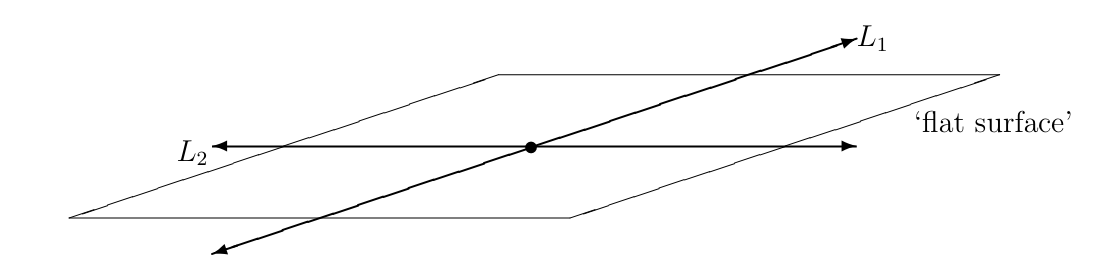
\includegraphics[width=0.7\textwidth]{figures/intersecting_lines.png}
    \caption{Two lines intersecting at a point lie on a unique plane.}
    \label{fig:intersecting-lines}
\end{figure}


  \item \textbf{Lines and Planes:} If a straight line intersects a flat surface in more than one point, then it must lie entirely within the surface. The figure below shows this situation: one line intersects the surface at a single point (and is not part of the plane), while another line intersects it in two points—indicating that it lies in the plane.
    \begin{figure}[htbp]
    \centering
    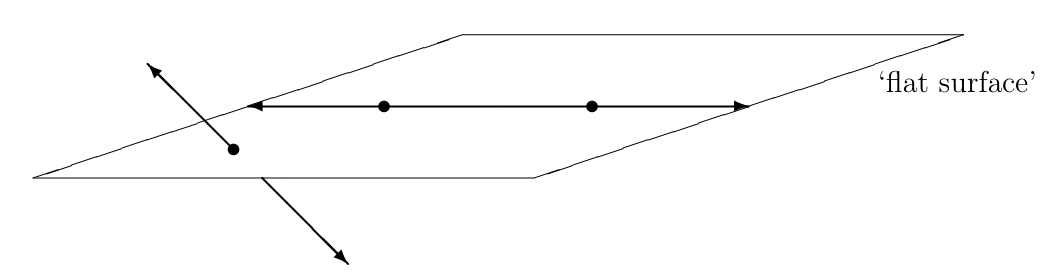
\includegraphics[width=0.7\textwidth]{figures/line_intersections_plane.png}
    \caption{A line intersecting a plane in one point vs. in two points.}
    \label{fig:line-plane-intersections}
\end{figure}

  

  \item \textbf{Three Points:} If we fix three points in space that do not all lie on the same line (i.e., they are \emph{non-collinear}), there is exactly one flat surface—one plane—that passes through all three. Imagine holding a rigid wooden board against a wall by three of its corners. The entire board is forced to lie flat against the wall; there's no room for bending. This illustrates the uniqueness of a plane determined by three non-collinear points.
        \begin{figure}[htbp]
    \centering
    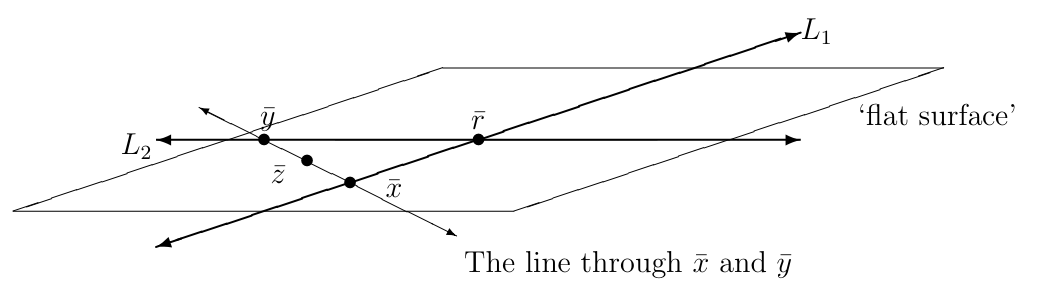
\includegraphics[width=0.6\textwidth]{figures/three_points_plane.png}
    \caption{A unique plane passes through three non-collinear points.}
    \label{fig:three-points-plane}
\end{figure}

\end{itemize}

\newpage

These intuitive ideas lead us toward a more formal definition of a plane in $\mathbb{R}^3$.

Now, suppose we are given two lines in space, $L_1$ and $L_2$, that intersect at a point $\bar{r}$. From earlier discussions (e.g., the theorem on intersecting lines), we know that these lines can be expressed parametrically as:
\[
\bar{x} = \bar{r} + t(\bar{p} - \bar{r}), \quad t \in \mathbb{R},
\]
\[
\bar{y} = \bar{r} + s(\bar{q} - \bar{r}), \quad s \in \mathbb{R},
\]
where $\bar{p} \in L_1$, $\bar{q} \in L_2$, and both pass through the common point $\bar{r}$. We now ask: what kind of surface contains \emph{every point} on both of these lines?

Take any point $\bar{x}$ on $L_1$ and any point $\bar{y}$ on $L_2$. The line connecting $\bar{x}$ and $\bar{y}$ lies in the same surface. A general point along this line can be described by:
\[
\bar{z} = \bar{x} + \alpha(\bar{y} - \bar{x}) = \bar{r} + (\alpha s)(\bar{q} - \bar{r}) + (t - \alpha t)(\bar{p} - \bar{r}), \quad \alpha \in \mathbb{R}.
\]

Thus, any such point $\bar{z}$ lies in the surface determined by $\bar{r}, \bar{p}, \bar{q}$. As we vary $s, t, \alpha \in \mathbb{R}$, we generate all points on this surface.

It appears reasonable, both geometrically and algebraically, that this set includes \emph{all} points on the plane determined by the intersecting lines $L_1$ and $L_2$.

\begin{definitionbox}

\textbf{Plane}

A \textit{plane} in \( \mathbb{R}^3 \) is a set
\[
P = \left\{ \bar{r} + s(\bar{p} - \bar{r}) + t(\bar{q} - \bar{r}) : s, t \in \mathbb{R} \right\}
\]
where \( \bar{p}, \bar{q}, \bar{r} \in \mathbb{R}^3 \) such that \( \bar{p} - \bar{r} \) and \( \bar{q} - \bar{r} \) are not scalar multiples of each other.
\end{definitionbox}

\begin{remarkbox}

Consider a set
\[
P = \left\{ \bar{r} + s(\bar{p} - \bar{r}) + t(\bar{q} - \bar{r}) : s, t \in \mathbb{R} \right\}, \quad \text{where } \bar{p}, \bar{q}, \bar{r} \in \mathbb{R}^3.
\]
\begin{enumerate}
    \item If \( \bar{p} - \bar{r} = \alpha(\bar{q} - \bar{r}) \) for some \( \alpha \in \mathbb{R} \), then
    \[
    P = \left\{ \bar{r} + s\left( \alpha(\bar{q} - \bar{r}) \right) + t(\bar{q} - \bar{r}) : s, t \in \mathbb{R} \right\}
      = \left\{ \bar{r} + (\alpha s + t)(\bar{q} - \bar{r}) : s, t \in \mathbb{R} \right\}.
    \]
    Therefore, in this case, the set \( P \) is a \textbf{line} in space.

    \item If \( \bar{p} - \bar{r} \) and \( \bar{q} - \bar{r} \) are not scalar multiples of each other, then \( P \) is a \textbf{plane} in \( \mathbb{R}^3 \). Note that:
    \[
    \bar{r} = \bar{r} + 0(\bar{p} - \bar{r}) + 0(\bar{q} - \bar{r}), \quad
    \bar{p} = \bar{r} + 1(\bar{p} - \bar{r}) + 0(\bar{q} - \bar{r}),
    \]
    \[
    \bar{q} = \bar{r} + 0(\bar{p} - \bar{r}) + 1(\bar{q} - \bar{r}).
    \]
    Thus, \( \bar{r} \in P \), \( \bar{p} \in P \), and \( \bar{q} \in P \). We therefore call \( P \) the \textbf{plane through} \( \bar{p} \), \( \bar{q} \), and \( \bar{r} \).

    \item If \( P \) is a plane, then a point \( \bar{x} \in \mathbb{R}^3 \) lies on the plane \( P \) if and only if
    \[
    \bar{x} = \bar{r} + s(\bar{p} - \bar{r}) + t(\bar{q} - \bar{r}) \quad \text{for some } s, t \in \mathbb{R}.
    \]
    We therefore speak of the plane described by the equation:
    \[
    \bar{x} = \bar{r} + s(\bar{p} - \bar{r}) + t(\bar{q} - \bar{r}).
    \]

    \item Let \( P = \left\{ \bar{r} + s(\bar{p} - \bar{r}) + t(\bar{q} - \bar{r}) : s, t \in \mathbb{R} \right\} \) be a plane through \( \bar{p}, \bar{q}, \bar{r} \), and let
    \[
    \bar{a} = \alpha(\bar{p} - \bar{r}), \quad \bar{b} = \beta(\bar{q} - \bar{r}),
    \]
    with \( \alpha, \beta \in \mathbb{R} \setminus \{0\} \). Then it follows that
    \[
    P = \left\{ \bar{r} + s\bar{a} + t\bar{b} : s, t \in \mathbb{R} \right\}.
    \]
    Conversely, if \( \bar{a}, \bar{b} \in \mathbb{R}^3 \) are nonzero vectors that are not scalar multiples of each other, then the set
    \[
    Q = \left\{ \bar{r} + s\bar{a} + t\bar{b} : s, t \in \mathbb{R} \right\}
    = \left\{ \bar{r} + s\left( (\bar{a} + \bar{r}) - \bar{r} \right) + t\left( (\bar{b} + \bar{r}) - \bar{r} \right) : s, t \in \mathbb{R} \right\}
    \]
    is a plane through the points \( \bar{r} \), \( \bar{r} + \bar{a} \), and \( \bar{r} + \bar{b} \).
\end{enumerate}
\end{remarkbox}

\begin{examplebox}
Consider the set \( P = \left\{ \langle 2, 3, -2 \rangle + s\langle 1, -4, 2 \rangle + t\langle 2, -3, 4 \rangle : s, t \in \mathbb{R} \right\} \), and
let \( \bar{r} = \langle 2, 3, -2 \rangle \), \( \bar{a} = \langle 1, -4, 2 \rangle \), and \( \bar{b} = \langle 2, -3, 4 \rangle \). Determine \( \bar{r} + \bar{a} \) and \( \bar{r} + \bar{b} \).

\vspace{0.5em}

\textbf{Solution}

\vspace{0.5em}

Since \( \bar{a} \) and \( \bar{b} \) are not scalar multiples
of each other, \( P \) is a plane through \( \bar{r} \), \( \bar{r} + \bar{a} = \langle 3, -1, 0 \rangle \), and \( \bar{r} + \bar{b} = \langle 4, 0, 2 \rangle \).
\end{examplebox}

\begin{examplebox}
Consider the set \( P = \left\{ \langle -1, 1, 6 \rangle + s\langle 2, 3, -5 \rangle + t\langle -6, -9, 15 \rangle : s, t \in \mathbb{R} \right\} \). Determine the points through which \( P \) is a line.

\vspace{0.5em}

\textbf{Solution}

\vspace{0.5em}

Since \( \langle -6, -9, 15 \rangle = -3\langle 2, 3, -5 \rangle \), we have:
\[
P = \left\{ \langle -1, 1, 6 \rangle + (s - 3t)\langle 2, 3, -5 \rangle : s, t \in \mathbb{R} \right\}
= \left\{ \langle -1, 1, 6 \rangle + \alpha\langle 2, 3, -5 \rangle : \alpha \in \mathbb{R} \right\}.
\]
Therefore, \( P \) is the line through \( \langle -1, 1, 6 \rangle \) and \( \langle 1, 4, 1 \rangle \).
\end{examplebox}

\begin{examplebox}
Consider the plane \( P = \left\{ \bar{r} + s(\bar{p} - \bar{r}) + t(\bar{q} - \bar{r}) : s, t \in \mathbb{R} \right\} \), where
\( \bar{x} = \langle 2, 0, 0 \rangle \) and \( \bar{y} = \langle 1, 2, 0 \rangle \) are given. Let \( \bar{r} = \langle 1, 1, 0 \rangle \), \( \bar{p} = \langle 0, 3, 1 \rangle \), and \( \bar{q} = \langle 1, 2, 1 \rangle \). Determine whether or not the points \( \bar{x} \) and \( \bar{y} \) lie on \( P \).

\vspace{0.5em}

\textbf{Solution}

\vspace{0.5em}

The point \( \bar{x} = \langle 2, 0, 0 \rangle \) is in \( P \) if and only if for some \( s, t \in \mathbb{R} \),
\[
\bar{x} = \bar{r} + s(\bar{p} - \bar{r}) + t(\bar{q} - \bar{r}) = \langle 1 - s, 1 + 2s + t, s + t \rangle
\]


By comparing components:
\[
\begin{aligned}
2 &= 1 - s \quad &\Rightarrow s &= -1 \\
0 &= 1 + 2s + t \quad &\Rightarrow t &= 1 \\
0 &= s + t \quad &\text{Check: } -1 + 1 = 0.
\end{aligned}
\]
So \( \bar{x} \in P \). Now check \( \bar{y} = \langle 1, 2, 0 \rangle \):
\[
\bar{y} = \bar{r} + s(\bar{p} - \bar{r}) + t(\bar{q} - \bar{r}) = \langle 1 - s, 1 + 2s + t, s + t \rangle.
\]

Compare components:
\[
\begin{aligned}
1 &= 1 - s \quad &\Rightarrow s &= 0 \\
2 &= 1 + 2s + t \quad &\Rightarrow t &= 1 \\
0 &= s + t = 0 + 1 = 1 \quad &\text{Contradiction}.
\end{aligned}
\]
Since no such \( s, t \in \mathbb{R} \) satisfy all equations, \( \bar{y} \notin P \).
\end{examplebox}

\newpage

It was mentioned at the beginning of this unit three properties that a 'flat surface' must satisfy.
We can motivate our definition of a plane in \(\mathbb{R}^3\) by showing that it satisfies the properties.

\begin{theorembox}
    \textbf{Line in a Plane}

    Let \(L\) be a line in \(\mathbb{R}^3\) and \(P\) be a plane in \(\mathbb{R}^3\) If \(L\) intersects \(P\) in more than one point,
    then \(L \subseteq P\); that is, every point on \(L\) lies on \(P\).
\end{theorembox}

\begin{proofbox}
    Let \(P = \left\{ \bar{r} + s(\bar{p} - \bar{r}) + t(\bar{q} - \bar{r}) : s, t \in \mathbb{R} \right\}\), and suppose that \(L\) intersects
    \(P\) in two points \(\bar{a} \text{ and } \bar{b}\). Then by the Theorem on Multiple Intersections of Lines,
    \[
    L = \left\{t\bar{a} + (1 - t)\bar{b} : t \in \mathbb{R}\right\}.
    \]

    Since \(\bar{a},\bar{b} \in P\), there exist distinct real numbers \(s_0,s_1,t_0,t_1\) such that
    \[
    \bar{a} = \bar{r} + s_0(\bar{p} - \bar{r}) + t_0(\bar{q} - \bar{r}) \text{ and } \bar{b} = \bar{r} + s_1(\bar{p} - \bar{r}) + t_1(\bar{q} - \bar{r}).
    \]

    Now consider a point \(\bar{x} \in L\) Then for some \(t \in \mathbb{R}\),
   \[
\begin{aligned}
\bar{x} &= t\bar{a} + (1 - t)\bar{b} \\
&= t\left[ \bar{r} + s_0(\bar{p} - \bar{r}) + t_0(\bar{q} - \bar{r}) \right] + (1 - t)\left[ \bar{r} + s_1(\bar{p} - \bar{r}) + t_1(\bar{q} - \bar{r}) \right] \\
&= [t + (1 - t)]\bar{r} + [ts_0 + (1 - t)s_1](\bar{p} - \bar{r}) + [tt_0 + (1 - t)t_1](\bar{q} - \bar{r}) \\
&= \bar{r} + [ts_0 + (1 - t)s_1](\bar{p} - \bar{r}) + [tt_0 + (1 - t)t_1](\bar{q} - \bar{r}).
\end{aligned}
\]
Hence \(\bar{x} \in P \text{ and therefore } L \subseteq P.\)
 \hfill $\qed$
\end{proofbox}
 
\begin{theorembox}

  \textbf{Unique Plane through Intersecting Lines}

  Let \(L_1\) and \(L_2\) be two lines in space that intersect at a single point. Then there is exactly one plane \(P\) that contains both lines; that is, 
  there is exactly one plane such that \(L_1 \subseteq P\) and \(L_2 \subseteq P\).

\end{theorembox}
        
\begin{proofbox}

We first show that there exists a unique plane \(P\) containing two intersecting lines \(L_1\) and \(L_2\).  

Assume \(L_1\) and \(L_2\) intersect at a point \(\bar{a}\), and let \(\bar{b} \in L_1\) and \(\bar{c} \in L_2\) be points different from \(\bar{a}\). Then, by the theorem on the intersection of lines, we hvae
\[
L_1 = \{\bar{a} + t(\bar{b}-\bar{a}) : t \in \mathbb{R}\}, \quad
L_2 = \{\bar{a} + s(\bar{c}-\bar{a}) : s \in \mathbb{R}\}.
\]

Now, consider any points \(x \in L_1\) and \(y \in L_2\). Then
\[
\bar{x} = \bar{a} + t_0(\bar{b}-\bar{a}), \quad \bar{y} = \bar{a} + s_0(\bar{c}-\bar{a})
\]
for some \(t_0, s_0 \in \mathbb{R}\). The vector connecting \(\bar{x}\) and \(\bar{y}\) is
\[
\bar{y} - \bar{x} = s_0(\bar{c}-\bar{a}) - t_0(\bar{b}-\bar{a}),
\]
which is a linear combination of \(\bar{b}-\bar{a}\) and \(\bar{c}-\bar{a}\). 

This implies that the vector connecting any point on \(L_1\) to any point on \(L_2\) lies in the span of \(\bar{b}-\bar{a}\) and \(\bar{c}-\bar{a}\). 
Consequently, if we start at \(\bar{a}\) and add all linear combinations of these two vectors, we obtain all points on \(L_1\), all points on \(L_2\), and all points “between” them. 
In other words, we obtain the entire plane containing both lines. Hence, the set
\[
P = \{\bar{a} + t(\bar{b}-\bar{a}) + s(\bar{c}-\bar{a}) : t, s \in \mathbb{R}\}
\]
contains both \(L_1\) and \(L_2\), so at least one plane containing them exists.

\vspace{1em}

Now we prove that said plane is unique.

By construction, \(\bar{b}-\bar{a}\) and \(\bar{c}-\bar{a}\) are not scalar multiples of each other, because \(L_1\) and \(L_2\) are distinct lines. 

According to the definition of a plane in \(\mathbb{R}^3\), a plane is uniquely determined by a point and two non-collinear vectors. 

Therefore, any plane containing the point \(\bar{a}\) and the vectors \(\bar{b}-\bar{a}\) and \(\bar{c}-\bar{a}\) must coincide with \(P\).  

Hence, the plane containing \(L_1\) and \(L_2\) is unique, and we have
\[
  P = \{\bar{a} + t(\bar{b}-\bar{a}) + s(\bar{c}-\bar{a}) : t, s \in \mathbb{R}\}.
\]

\hfill $\qed$

\end{proofbox}

\begin{examplebox}
  Consider the lines \(L_1\) and \(L_2\) through \(\bar{p} = \langle 1,0,1 \rangle\) and \(\bar{q} = \langle 1,2,-2 \rangle\),
  and \(\bar{u} = \langle -1,2,0 \rangle\) and \(\bar{v} = \langle -3,3,0 \rangle\).

  Show that \(L_1\) and \(L_2\) intersect, and find an equation for the plane containing both lines.

  \vspace{0.5em}

  \textbf{Solution}

  \vspace{0.5em}

  \(L_1\) and \(L_2\) intersect at \(\bar{a} = \langle x, y, z \rangle\) if and only if
  \[
    \bar{q} + t(\bar{p} - \bar{q}) = \bar{a} = \bar{u} + s(\bar{v} - \bar{u})
    \quad \text{for some } t, s \in \mathbb{R},
  \]
  \[
    \text{i.e.,}
  \]
  \[
    1 = x = 2s - 3,\quad
    2 - 2t = y = 3 - s,\quad
    2t - 1 = z = 0
    \quad \text{for some } s, t \in \mathbb{R}.
  \]
  The first equation implies \(s = 2\), and the third that \(t = \tfrac{1}{2}\).
  These values for \(s\) and \(t\) also satisfy the second equation.
  Therefore the lines \(L_1\) and \(L_2\) intersect at the point
  \[
    \bar{a} = \tfrac{1}{2} \bar{p} + \left( 1 - \tfrac{1}{2} \right) \bar{q}
    = \langle 1, 1, 0 \rangle.
  \]

  According to the Theorem on a Unique Plane through Intersecting Lines, there is exactly one plane \(P\) containing both \(L_1\) and \(L_2\).

  In order to write down an equation for this plane, we need three points on the plane that are not all on the same line.

  We have \(\bar{a} \in L_1\), \(\bar{a} \in L_2\), \(\bar{p} \in L_1\), \(\bar{u} \in L_2\).

  Since \(P\) contains \(L_1\) and \(L_2\), it follows that \(\bar{a}, \bar{p}, \bar{u} \in P\).
  
  But \(\bar{p} \notin L_2\) and \(\bar{u} \notin L_1\).
  Therefore \(\bar{a}, \bar{p}, \bar{u}\) are not all on the same line.

  Hence an equation for \(P\) is
  \[
    \bar{x} = \bar{a} + s(\bar{p} - \bar{a}) + t(\bar{u} - \bar{a})
    = \langle 1, 1, 0 \rangle + s\langle 0, -1, 1 \rangle + t\langle -2, 1, 0 \rangle.
  \]
\end{examplebox}


\begin{theorembox}

  \textbf{Three-Point Plane Theorem}

  Let \(\bar{p}, \bar{q}\) and \(\bar{r}\) be three points in \(\mathbb{R}^3\), not all on the same line. 
  Then there exists a unique plane \(P \in \mathbb{R}^3\) such that \(\bar{p}, \bar{q}, \bar{r} \in P\).
\end{theorembox}

\begin{proofbox}
  Let \(L_1\) be the line through \(\bar{p}\) and \(\bar{r}\), and \(L_2\) be the line through \(\bar{q}\) and \(\bar{r}\).

  \vspace{0.5em}

  Since \(\bar{p}, \bar{q}\) and \(\bar{r}\) are not all on the same line, it follows that \(L_1\) and \(L_2\) intersect at a single point, namely, at \(\bar{r}\).
  It follows from the Theorem on a Unique Plane through Intersecting Lines that there exists a unique plane \(P\) containing both \(L_1\) and \(L_2\).

  \vspace{0.5em}

  Since \(\bar{p},\bar{r} \in L_1\) and \(\bar{q},\bar{r} \in L_2\), it follows that \(\bar{p},\bar{q},\bar{r} \in P\).

  \vspace{0.5em}

  If some plane \(Q\) is a plane containing \(\bar{p},\bar{q},\) and \(\bar{r}\), then \(L_1,L_2 \subseteq Q\) by the Theorem on a Line in a Plane
  Since \(P\) is the unique plane containing both \(L_1\) and \(L_2\), it follows that \(P = Q\). 

  \hfill \(\qed\)

\end{proofbox}

\newpage

Recall that we call two lines \(L_1 = \{\bar{q} + t(\bar{p} - \bar{q}) : t \in \mathbb{R}\}\) and \(L_2 = \{\bar{r} + s(\bar{q} - \bar{r}) : s \in \mathbb{R}\}\)
\textit{parallel} if \(\bar{p} -\bar{q}\) and \(\bar{a}-\bar{b}\) are scalar multiples of each other. We showed in the Theorem on the Non-Intersection of Parallel Lines that
if \(L_1\) and \(L_2\) are parallel, and \(L_1 \neq L_2\), then \(L_1\) and \(L_2\) do not intersect. The converse of this statement is false-in the example that followed, we showed an instance
of two lines that are not parallel, and do not intersect. 

The following result further clarifies this issue.

\begin{theorembox}

  \textbf{Parallel Lines in a Plane}

Let \(L_1\) and \(L_2\) be two lines in \(\mathbb{R}^3\) such that \(L_1 \neq L_2\) defined as

\[
  L_1 = \{\bar{q} + t(\bar{p} - \bar{q}) : t \in \mathbb{R}\}, \quad
  L_2 = \{\bar{r} + s(\bar{q} - \bar{r}) : s \in \mathbb{R}\}.
\]

Then the following statements are true:
\begin{enumerate}[label=(\arabic*)]
  \item If \(L_1\) and \(L_2\) are parallel, then there exists exactly one plane \(P\) that contains both lines.
  \item If \(L_1\) and \(L_2\) do not intersect, and there is a plane \(P\) such that \(L_1,L_2 \subseteq P\), then \(L_1\) and \(L_2\) are parallel.
\end{enumerate}
\end{theorembox}

\begin{proofbox}

  \begin{enumerate}[label=(\arabic*), series = ParLinProof]
    \item Assume that \(L_1\) and \(L_2\) are parallel. Then by the definition of parallel lines, there exists a non-zero \(\alpha \in \mathbb{R}\) such that

    \[
      \bar{a} - \bar{b} = \alpha(\bar{p} - \bar{q}).
    \]

    Since \(L_1\) and \(L_2\) are parallel, it follows by the Theorem on Non-Intersection of Parallel Lines, that \(L_1\) and \(L_2\) do not intersect.

    Therefore \(\bar{p},\bar{q}, \bar{b}\) are not all on the same line. By the Three-Point Plane Theorem, we find that

    \[
      P = \{\bar{q} + s(\bar{p} - \bar{q}) + t(\bar{b} - \bar{q}) : s, t \in \mathbb{R}\}.
    \]
    is a plane in \(\mathbb{R}^3\) such that \(\bar{p}, \bar{q}, \bar{b} \in P\).

    Now consider points \(\bar{x}\) and \(\bar{y}\) on \(L_1\) and \(L_2\), respectively.

    Then
    \[
      \bar{x} = \bar{q} + t(\bar{p} - \bar{q}), \quad
      \bar{y} = \bar{r} + s(\bar{q} - \bar{r}) \text{ for some s,t } \in \mathbb{R}.
    \]


  \end{enumerate}
\end{proofbox}
\end{document}